% Quantum Krylov chemistry on Quantinuum hardware: merged document.
% Formed on 2026-10-15 by merging a reviewer's report on the SKQD report (flaws, alternatives, publication
% strategy) with a claim-by-claim check of the "four state-of-the-art paradigms" brief; the two source
% documents were removed afterwards. All toy numerics come from one script: code/krylov_toy_checks_h2.py.
% Style: workspace mathnotes.sty (plain academic, text colour only).
% Build:  ../../tools/build-tex.sh quantinuum-krylov-review-and-strategy.tex
\documentclass[11pt,a4paper]{article}
\usepackage{mathnotes}
\usepackage{tabularx}
\newcolumntype{Y}{>{\raggedright\arraybackslash}X}
\newcolumntype{L}[1]{>{\raggedright\arraybackslash}p{#1}}
\setcounter{tocdepth}{1}
\setlength{\parindent}{0pt}
\setlength{\parskip}{5pt}
\setlist[itemize]{itemsep=2pt,topsep=3pt}
\setlist[enumerate]{itemsep=3pt,topsep=3pt}
\graphicspath{{../}}

\newcommand{\ket}[1]{\lvert #1\rangle}
\newcommand{\bra}[1]{\langle #1\rvert}
\newcommand{\braket}[2]{\langle #1\vert #2\rangle}
\newcommand{\ex}[1]{\langle #1\rangle}
\newcommand{\Hd}{H_{\mathrm{drive}}}
\newcommand{\Ht}{H_{\mathrm{full}}}
\newcommand{\mHa}{\,\mathrm{mHa}}
\newcommand{\Ha}{\,\mathrm{Ha}}
\newcommand{\HQC}{\mathrm{HQC}}
\newcommand{\report}{the report}
% evidence labels
\newcommand{\lR}{\textcolor{keyblue}{[R]}}   % verified from the SKQD report text
\newcommand{\lP}{\textcolor{keyblue}{[P]}}   % a claim made in the "four paradigms" brief
\newcommand{\lV}{\textcolor{keyblue}{[V]}}   % verified in this workspace (Hiverge paper, web check 2026-10-15)
\newcommand{\lA}{\textcolor{notegray}{[A]}}  % own reasoning / analysis
\newcommand{\lG}{\textcolor{alertred}{[G]}}  % general knowledge: verify before citing
\newcommand{\lN}{\textcolor{keyblue}{[N]}}   % numerical check in code/krylov_toy_checks_h2.py
\newcommand{\sev}[1]{\textbf{Severity: #1.}}
% Call-out paragraphs: plain indented text with a coloured run-in title (no boxes or frames).
\newenvironment{idea}[1][Main idea]{\par\smallskip\begin{quotation}\noindent{\bfseries\textcolor{keyblue}{#1.}}\ }{\end{quotation}\smallskip}
\newenvironment{caution}[1][Caution]{\par\smallskip\begin{quotation}\noindent{\bfseries\textcolor{alertred}{#1.}}\ }{\end{quotation}\smallskip}
\newcommand{\takeaway}[1]{\par\smallskip\noindent{\bfseries\textcolor{keyblue}{Takeaway.}} #1\par\smallskip}
\newcommand{\verdict}[1]{\par\smallskip\noindent{\bfseries\textcolor{keyblue}{Verdict for our paper.}} #1\par\smallskip}
% a flaw entry: \flaw{id}{title}{where}{severity}
\newcommand{\flaw}[4]{\par\medskip\noindent\textbf{#1 -- #2.}\quad{\small\textcolor{notegray}{Where: #3.}}\quad\sev{#4}\par\nobreak}

\title{Quantum Krylov chemistry on Quantinuum hardware\\\large Review of the SKQD report, the four ground-state paradigms checked, and a publication strategy}
\author{Prajjwal}
\date{15 October 2026}

\begin{document}
\maketitle

\begin{center}\small
\emph{What the report claims} $\cdot$ \emph{where the evidence is thin} $\cdot$ \emph{which paradigms are real on today's hardware} $\cdot$ \emph{what to do instead} $\cdot$ \emph{how to make it a Quantinuum paper}
\end{center}

\section*{How to read this document}
\addcontentsline{toc}{section}{How to read this document}
This document merges two earlier ones: a reviewer's report on ``Scalable Non-Iterative Quantum Krylov Subspace Chemistry on Trapped-Ion Processors'' (A.~Kumar, 8 October 2026, 14 pp.; ``\report'' below), and a claim-by-claim check of a brief that lists four ``state-of-the-art paradigms'' for molecular ground states on Quantinuum hardware (``the brief''). It is written for a first-time reader: the glossary (\cref{sec:glossary}) defines every acronym, each section ends with a one-line takeaway, and the toy numerics are gathered in one place (\cref{sec:numerics}) and produced by one script.

Every factual statement carries a label so that you can check it yourself:
\begin{itemize}
\item \lR\ \textbf{verified from the report text}: a page, equation, table or figure is cited (e.g.\ ``p.~8, Eq.~(32)'').
\item \lP\ \textbf{a claim made in the brief}, reproduced so that it can be checked.
\item \lV\ \textbf{verified in this workspace}: from the Quantinuum/Hiverge preprint in this folder, from the project notes, or from a web check made on 15 October 2026 (Quantinuum's HQC formula; the System Model H2 product page).
\item \lA\ \textbf{my own reasoning}: an inference from what a source says, or from standard linear algebra and cost arithmetic.
\item \lG\ \textbf{general knowledge, to be verified}: a fact about the literature or the hardware that I believe to be correct but that you must confirm before quoting it in a paper.
\item \lN\ \textbf{numerical check}: a result of \texttt{code/krylov\_toy\_checks\_h2.py}, a statevector toy on the 2-qubit H$_2$ model with Gaussian shot noise. It illustrates mechanisms; it is \alert{never a hardware result}.
\end{itemize}
{\sloppy The model for a credible Quantinuum hardware paper is the Quantinuum/Hiverge preprint ``Automated near-term quantum algorithm discovery for molecular ground states'' (arXiv:2603.26359, March 2026), cited as ``the Hiverge paper''. The companion documents \texttt{qite-complete-guide.pdf} (QITE from first principles, with the QITE-versus-Krylov benchmark idea) and \texttt{Krylov\_SKQD\_Study\_Notes.pdf} (your own study of \report) are referred to rather than repeated.\par}

\section*{Executive summary}
\addcontentsline{toc}{section}{Executive summary}
\textbf{The report.} It presents a pipeline for molecular ground-state energies on Quantinuum H2-1/H2-2: exact $\mathbb{Z}_2$ tapering (12 to 7--8 qubits), perturbative pruning of the Hamiltonian, ancilla-free ``sample-based Krylov quantum diagonalisation'' (SKQD) in which the quantum computer only proposes computational-basis bitstrings and a classical computer diagonalises the full Hamiltonian in the span of those bitstrings, and a two-tier statistical filter for noisy bitstrings. It reports chemical accuracy for H$_2$O (hardware, 0.11--0.31\,mHa), F$_2$ (hardware, ``0.0000\,mHa'') and four further molecules in six-orbital active spaces, and claims a ``100\% chemical accuracy pass rate''. The hardware runs are real and the exposition of tapering and of the method's scaling ``walls'' is honest and useful. But the paper does not show that the quantum computer contributed anything, and its evidence is unquantified.

\textbf{Top five flaws} (details in \cref{sec:flaws}):
\begin{enumerate}
\item \textbf{The classical step does the work; no classical control} (F7, F8). 249/256 basis states for water; $\le 400$ determinants in every active space; raw noisy hardware beats both the filtered run and the noiseless simulator. Nothing isolates a quantum contribution.
\item \textbf{Novelty and framing} (F24). The method is SKQD/SQD/QSCI from the 2023--25 literature, uncited; the ``Defense of Supremacy'' section claims a milestone that no $\le 8$-qubit calculation can support.
\item \textbf{No statistics, no reproducibility} (F13, F22). One hardware run per molecule, no error bars, no bootstrap, no raw counts, no code, no Hamiltonians, no software versions. Compare the Hiverge paper: $10^4$ shots, bootstrap, ``$3.1 \pm 3.4$\,mHa'', public repository.
\item \textbf{Resource accounting is wrong} (F19, F20). Eq.~(9) is not Quantinuum's HQC formula, Eq.~(10) uses a different denominator from Eq.~(9), the batch total is not $6\times$ the per-circuit cost, and no actual HQC, wall-time or classical cost is reported.
\item \textbf{Theory claims that do not hold for the implemented method} (F1, F2, F6). The Krylov convergence story does not apply to a compact 10--30-term driver; ``every omitted term is fully restored'' is false in general; the two-tier filter discards exactly the rare configurations the paper's own ``sampling wall'' says are the bottleneck.
\end{enumerate}

\textbf{The four paradigms in the brief} (details in \cref{sec:p1,sec:p2,sec:p3,sec:p4}):
\begin{enumerate}
\item \textbf{QPE with low-rank factorisation (DF/THC, iterative QPE)}: correct as the fault-tolerant end-point, irrelevant to a 500--5\,000 HQC budget. One-ancilla iterative QPE trades qubits for coherent evolution growing as $2^{m}$ for $m$ bits; the toy needs 2\,048 units of controlled evolution for 12 bits (\lN). One line in a cost table, no runs.
\item \textbf{Krylov / QLanczos}: the right family and already our backbone; the brief's ``Quantinuum heavily favours it'' is unsupported, its swap-network sentence is backwards on an all-to-all device, and it omits the two deciding issues: Hadamard-test shot cost and the conditioning of the overlap matrix (both measured in \cref{sec:numerics}).
\item \textbf{ADAPT-VQE and generative ans\"atze}: ADAPT correctly described; the ``transformer trained on molecular graphs, $10\times$ faster'' story conflates the Hiverge paper (LLM-driven evolutionary \emph{algorithm discovery}) with the separate generative-eigensolver line and is unsourced. State preparation and baseline, not the novelty.
\item \textbf{Fault-tolerant GSEE / statistical phase estimation / syndromes}: three things bundled. Statistical phase estimation is \emph{near-term} and, on the toy, reaches chemical accuracy in 100\% of runs at $10^5$ shots per time point where coherent Krylov from the same data reaches 55\% (\lN); logical-qubit chemistry is out of scope; stabiliser syndromes and symmetry post-selection are different tools and only the second is available to us.
\end{enumerate}

\textbf{Top three recommendations} (details in \cref{sec:strategy}):
\begin{enumerate}
\item \textbf{Reframe as a budget-matched, four-arm benchmark}, not a supremacy claim: sample-based diagonalisation (SKQD/SQD with the full driver), coherent Krylov with error-detected overlaps, QITE/QLanczos, and statistical phase estimation (free: it re-uses the coherent-Krylov data), plus classical-only controls, on active spaces of 12--20 orbitals where the connected expansion cannot saturate. The central figure is energy error (with confidence intervals) versus cumulative hardware cost.
\item \textbf{Adopt the Hiverge reporting standard}: emulator first (raw, symmetry-verified, forecast noise), then hardware; $\ge 3$ independent repeats; bootstrap intervals; native-gate ledger per circuit; public code, Hamiltonians and raw counts; explicit device, dates and software versions.
\item \textbf{Make the quantum part matter and use the hardware's strengths}: a full-Hamiltonian Trotter driver (so the SKQD guarantee applies), residual-guided selection and adaptive shot allocation, and mid-circuit-measurement-based symmetry/error detection with qubit reuse, because that is what superconducting-platform SQD papers cannot do. Co-design with Quantinuum (InQuanto, Nexus, H2-1E/H2-2E emulators). Do not add QPE or logical-qubit work.
\end{enumerate}

\clearpage
{\setlength{\parskip}{0pt}\tableofcontents}
\clearpage

%=====================================================================================
\part{Background}

\section{Glossary}\label{sec:glossary}
\begin{center}\small
\begin{tabularx}{\linewidth}{@{}L{3.4cm}Y@{}}
\toprule
Term & Plain-language meaning\\\midrule
Ground state, $E_0$ (GSEE) & The lowest-energy electronic state of a molecule and its energy; ``ground-state energy estimation'' is the task of finding $E_0$. The target of everything here.\\
Chemical accuracy & Energy error below $1\,\mathrm{kcal/mol}\approx1.6\,\mathrm{mHa}$ ($1\,\mathrm{mHa}=10^{-3}$ Hartree). Usually measured against an exact reference \emph{in the same model}; it says nothing about agreement with experiment.\\
HF & Hartree--Fock: the best single-determinant (mean-field) state. Cheap, usually the starting point, misses correlation.\\
FCI / CASCI & Full configuration interaction: the exact answer in a chosen orbital basis. CASCI is FCI inside a small ``active space'' of orbitals (e.g.\ CAS(8e,6o) = 8 electrons in 6 orbitals) with the rest frozen.\\
Active space & The handful of orbitals and electrons treated quantum mechanically; everything else is frozen classically. Fixes the qubit count ($2\times$ spatial orbitals before tapering).\\
CCSD(T), MP2 & Coupled cluster with singles, doubles and perturbative triples: the classical ``gold standard'' for weakly correlated molecules. MP2 is cheaper second-order perturbation theory. Both fail when several determinants are equally important (strong correlation).\\
DMRG, SCI, SHCI, HCI & Classical methods for strongly correlated systems: density-matrix renormalisation group; selected CI (keep only important determinants); semistochastic/heat-bath CI are modern SCI variants. These are the honest classical competitors.\\
Determinant / bitstring & An occupation pattern of spin-orbitals. After the Jordan--Wigner map, a computational-basis bitstring of the qubits. The ground state is a weighted sum of such bitstrings.\\
Pauli string, $\lambda$ & $H=\sum_m h_m P_m$ with $P_m$ tensor products of $I,X,Y,Z$. The 1-norm $\lambda=\sum_m|h_m|$ sets the cost of block-encoding methods.\\
Tapering & Removing qubits exactly by exploiting $\mathbb{Z}_2$ symmetries (particle-number parity, point group). Zero error by construction.\\
Trotter step, $e^{-iHt}$ & Approximating real-time evolution as a product of short gates, one per Hamiltonian term. Error grows with $t$ and with non-commuting terms; controlled by the number of steps $r$.\\
Quantum Krylov (QKS/QKSD) & Build a basis $\{e^{-iHt_k}\ket{\mathrm{HF}}\}$, measure the overlap matrix $\mathbf S$ and Hamiltonian matrix $\mathbf H_K$ between these states, solve $\mathbf H_K c=E\,\mathbf S c$. ``Coherent'' Krylov in this document.\\
Hadamard test & One-ancilla circuit that returns $\operatorname{Re}$ or $\operatorname{Im}$ of $\bra{\psi_0}U\ket{\psi_0}$ from the ancilla statistics. Needs controlled-$U$. How coherent Krylov gets its matrix elements.\\
Conditioning, $\kappa(\mathbf S)$ & Ratio of largest to smallest eigenvalue of $\mathbf S$. When Krylov vectors are nearly parallel, $\kappa$ explodes and shot noise is amplified; one must drop small eigenvalues (thresholding / canonical orthogonalisation) or add a ridge.\\
SKQD & Sample-based Krylov quantum diagonalisation: run the Krylov circuits but only \emph{measure bitstrings}; then diagonalise $H$ classically in the span of the sampled bitstrings. The overlap matrix is the identity ($\mathbf S=I$). Introduced by Yu et al.\ (2025) \lG.\\
SQD / QSCI & Sample-based quantum diagonalisation (IBM, 2024--25) and quantum-selected CI (Kanno et al., 2023): same idea as SKQD but the bitstrings come from any prepared state, with classical ``configuration recovery'' of noisy samples \lG.\\
Connected expansion & Classical step: add every bitstring coupled by $H$ to an already selected one. One ``shell'' of this from HF alone generates all single and double excitations.\\
\bottomrule
\end{tabularx}
\end{center}
\begin{center}\small
\begin{tabularx}{\linewidth}{@{}L{3.4cm}Y@{}}
\toprule
Term & Plain-language meaning\\\midrule
QITE / QLanczos & Quantum imaginary-time evolution: approximate the cooling map $e^{-\tau H}$ by measured, state-dependent unitaries; QLanczos builds a Krylov space from QITE states. Iterative (needs feedback). See \texttt{qite-complete-guide.pdf}.\\
VQE, HEA, ADAPT-VQE & Variational quantum eigensolver: optimise circuit angles to minimise energy. HEA = hardware-efficient ansatz (shallow, symmetry-breaking). ADAPT grows the circuit one operator at a time from a pool using energy gradients. The Hiverge paper's baselines.\\
QPE, IQPE & Quantum phase estimation: read the eigenphase of $e^{-iHt}$ into an ancilla register. Iterative (Kitaev) QPE uses one ancilla and reads one binary digit per round.\\
Block encoding, qubitisation & Embedding $H/\lambda$ in a unitary; the ``walk operator'' $W$ has eigenphases $\pm\arccos(E_n/\lambda)$, so QPE on $W$ gives $E_n$. The standard fault-tolerant route.\\
DF, THC & Double factorisation and tensor hypercontraction: low-rank rewritings of the two-electron integrals that shrink $\lambda$ and the gates needed to build $W$.\\
SPE, QCELS, RPE & Statistical / robust phase estimation: measure the signal $s(t)=\bra{\psi_0}e^{-iHt}\ket{\psi_0}$ at several $t$ and fit frequencies classically (Fourier, Prony, matrix pencil, least squares). No eigenproblem, one ancilla, much better shot scaling.\\
Shots & Repetitions of a circuit. Averages have noise $\sim 1/\sqrt{N_{\rm shots}}$; a bitstring with probability $p$ needs $\sim 1/p$ shots to be seen once.\\
Depth, 2Q gates & Circuit depth = number of sequential gate layers; two-qubit (2Q) gate count = number of native entangling gates (ZZPhase on Quantinuum). Both drive error and cost on hardware.\\
$R_{ZZ}(\theta)$, ZZPhase & Quantinuum's native arbitrary-angle two-qubit gate $\exp(-i\tfrac\theta2 Z\otimes Z)$.\\
MCMR, qubit reuse & Mid-circuit measurement and reset: measure some qubits during a circuit and act on the result (detect an error and discard the shot, or reset and reuse the qubit). A distinctive trapped-ion capability.\\
PMSV & Partition-measurement symmetry verification (InQuanto): discard shots that violate a known symmetry (particle number, spin). Cheap error detection used in the Hiverge paper.\\
Error detection code & A small code (e.g.\ Iceberg $[[k{+}2,k,2]]$) that flags, but does not correct, single errors; flagged shots are discarded.\\
Logical qubit & A qubit encoded in many physical qubits with error correction. Current demonstrations: a few to a few tens of logical qubits.\\
HQC & Hardware quantum credit, Quantinuum's usage unit: $\HQC=5+C\,(N_{1q}+10N_{2q}+5N_m)/5000$ per circuit with $C$ shots (\lV). \emph{Not} a currency.\\
H2-1, H2-2, H2-1E, Helios & Quantinuum System Model H2 machines (56 trapped-ion qubits, all-to-all connectivity), their emulators (``E''), and the 2025 successor Helios (98 qubits) \lG.\\
Emulator / statevector & Emulator: a classical simulation with a device noise model. Statevector: exact noiseless simulation.\\
\bottomrule
\end{tabularx}
\end{center}

\section{The hardware premises, checked}\label{sec:hardware}
The brief opens with four hardware facts \lP: all-to-all connectivity, two-qubit error $\sim10^{-3}$--$10^{-4}$, mid-circuit measurement and reset, and native arbitrary-angle $R_{ZZ}$. What we can actually stand on:

\begin{center}\small
\begin{tabularx}{\linewidth}{@{}L{3.6cm}YY@{}}
\toprule
Claim in the brief & Status & Comment\\\midrule
All-to-all connectivity & \lV\ (H2 product page) & Ions are physically shuttled; any pair can interact. No SWAP routing cost, which matters for Pauli strings of high weight and for non-local encodings.\\
2Q error $10^{-3}$--$10^{-4}$ & \lV\ for $\sim10^{-3}$ ($>99.9\%$ fidelity on H2); \lG\ for anything approaching $10^{-4}$ & Helios is reported at $99.92\%$ in press coverage ($8\times10^{-4}$). Plan with $10^{-3}$; treat $10^{-4}$ as not yet available.\\
Mid-circuit measurement, reset, conditional logic & \lV & The ingredient that distinguishes a Quantinuum paper; see \cref{sec:p4}.\\
Native $R_{ZZ}(\theta)$ & \lV\ (ZZPhase is the native gate named in \report\ and the Hiverge paper) & Saves gates for \emph{weight-2} Pauli rotations; the brief's ``halving'' is overstated for general Pauli gadgets (\cref{sec:pipeline}).\\
Qubit counts & \lV\ 56 (H2); \lG\ 98 (Helios) & Far more than an 8--20 qubit active space needs; the binding constraint is HQC budget and 2Q count, not qubits.\\
Emulators and mitigation & \lV\ (Hiverge paper, Sec.~5.4) & H2-1E/H2-2E with device noise models and the PMSV mitigation exist in InQuanto.\\
\bottomrule
\end{tabularx}
\end{center}

\begin{idea}[What the budget really is]
\report\ says a typical academic allocation is 500--5\,000 HQC \lR. With the published formula, one 8-qubit Hadamard-test circuit with 300 two-qubit gates costs $734\,\HQC$ at $10^3$ shots and $7\,295\,\HQC$ at $10^4$ shots (\lN, Check~G). \emph{A single well-sampled Hadamard-test circuit can consume the whole budget.} Every paradigm below must be judged against this number, not against qubit counts.
\end{idea}

\takeaway{Connectivity, MCMR and the native gate are real; the $10^{-4}$ error figure is not yet. The constraint that decides everything is the HQC cost of two-qubit gates times shots.}

%=====================================================================================
\clearpage
\part{The SKQD report under review}

\section{What the report does and claims}\label{sec:summary}
\subsection{The pipeline in plain language}
The report (14 pages, 12 references) chains four ``reductions'' \lR:
\begin{enumerate}
\item \textbf{Tapering} (Sec.~3.2, pp.~5--6): find the Pauli operators that commute with every term of $H$ by Gaussian elimination over $\mathbb{F}_2$ (Eqs.~16--19), rotate them to single-qubit $X$'s with a Clifford (Eqs.~20--21), and replace each by its eigenvalue $\pm1$ (Eq.~22). 12 qubits become 7--8. This is exact.
\item \textbf{Pruning the driver} (Sec.~3.3, pp.~6--7): keep all diagonal ($I/Z$) terms (``Rule 1'', Eq.~25) and drop off-diagonal terms whose second-order Epstein--Nesbet energy $|c_k|^2/\Delta E_{\rm gap}$ is below $\eta=10^{-7}$\,Ha (Eq.~26).
\item \textbf{Ancilla-free SKQD} (Sec.~3.4, pp.~7--8): keep only the $K\in[10,30]$ largest off-diagonal terms plus the diagonal as a ``compact driving operator'' $\Hd$ (Eq.~30), evolve $\ket{\Phi_{\rm HF}}$ under $e^{-i\Hd t_k}$ for $t_k\in\{0,0.15,\dots,0.75\}$ (Eq.~31), and measure bitstrings. Because bitstrings are orthonormal, $\mathbf S=I$ (Eq.~32). Classically, add every bitstring coupled by $\Ht$ to a sampled one (``connected expansion'', Eq.~33) and diagonalise $\Ht$ in that space (Eq.~34).
\item \textbf{Two-tier filter} (Sec.~3.5, pp.~8--9): discard bitstrings seen fewer than $N_{\min}=2$ times or with frequency below $\nu_{\min}=0.1\%$ (Eq.~35), and bitstrings whose second-order coupling to HF is below $10^{-6}$\,Ha (Eq.~36).
\end{enumerate}

\subsection{The reported numbers}
\begin{center}\small
\begin{tabularx}{\linewidth}{@{}L{2.6cm}L{1.5cm}rrrrY@{}}
\toprule
Case & Where & Qubits & 2Q & Depth & Err.\ (mHa) & Provenance stated\\\midrule
H$_2$O, raw & p.~10, Tab.~1 & 8 & 150 & 428 & 0.1113 & H2-1 hardware, job ID given, $6\times1024$ shots\\
H$_2$O, filtered & p.~10, Tab.~1 & 8 & 150 & 428 & 0.3095 & same job, 53 core $\to$ 249 expanded states\\
H$_2$O, statevector & p.~10, Tab.~1 & 8 & 150 & 428 & 0.1836 & noiseless\\
H$_2$O, emulator & p.~10, Tab.~1 & 8 & 150 & 428 & 0.1836 & H2-1E, 1024 shots\\
``Standard QKS'' & p.~10, Tab.~1 & 12 & 5436 & 18572 & $>50$ & ``decoheres''; no run described\\
F$_2$ & p.~10, Tab.~2 & 7 & 153.3 (avg.) & 505 & 0.0000 & H2-2 hardware; no job ID, no shots stated\\
N$_2$, CH$_4$ & p.~11, Tab.~3 & 7, 8 & 140, 110 & -- & 0.2854, 0.0016 & not stated\\
C$_2$H$_4$ (11 angles) & p.~11 & 4 & 40 & 162 & 0.0000 & not stated\\
C$_6$H$_6$ (9 geometries) & p.~11 & 7--8 & 204 & 698 layers & 0.0012 & ``compilation on H2-1'', ``1024-shot sampling''\\
\bottomrule
\end{tabularx}
\end{center}
All errors are relative to CASCI in the stated active space (STO-3G; all active spaces have $\le 6$ orbitals) \lR.

\subsection{The claims}
From the abstract and Sec.~7 \lR: (i) tapering with ``mathematically exact 0.0000\,mHa error''; (ii) pruning with $<0.1$\,mHa error; (iii) 2Q-gate reduction ``by up to 97.6\%'' and ``survival fidelity from $<0.03\%$ to $>80\%$''; (iv) chemical accuracy on hardware for H$_2$O and F$_2$; (v) a ``100\% chemical accuracy pass rate'' across six molecules; (vi) that ``classical single-reference methods (MP2 and CCSD) fail'' where the method succeeds; and (vii) Sec.~7.1, titled ``Defense of Supremacy'', lists four ``milestones''.

\takeaway{The report is a hardware demonstration of a sample-based diagonalisation workflow on tiny active spaces. The question a referee will ask first is: \emph{what did the quantum computer contribute that Hartree--Fock plus a classical expansion would not have?}}

\section{What a credible Quantinuum hardware paper looks like}\label{sec:hiverge}
The Hiverge paper is a useful yardstick because it reports VQE-type circuits on the same hardware family and was written with Quantinuum's hardware team. The table lists what it does and whether \report\ does the same \lR.
\begin{center}\small
\begin{tabularx}{\linewidth}{@{}L{3.6cm}YY@{}}
\toprule
Practice & Hiverge paper & The report\\\midrule
Baselines run by the authors, same pool/setting & ADAPT-VQE and QEB-ADAPT-VQE implemented in the same codebase, same operator pools (Sec.~5.1, App.~A.3) & None run. ``Standard QKS'' row is an unexecuted estimate; MP2/CCSD failure is quoted from another paper\\
Resource reporting & Per-geometry parameters, circuit evaluations, 2Q gates after compilation to the H2 native gate set (Fig.~5) & Single 2Q count and depth per molecule; no shots/HQCs/time ledger\\
Noise study before hardware & H2-1 emulator in three regimes: raw, PMSV-mitigated, ``forecast'' with tuned error rates (Fig.~7) & One 1024-shot emulator energy, noise model not described\\
Hardware statistics & $10^4$ shots per circuit, bootstrap error bars, result quoted as $3.1\pm3.4$\,mHa, ``statistically consistent with chemical precision'' (Sec.~5.4) & 1024 shots per circuit, one run, no uncertainty, errors quoted to $10^{-4}$\,mHa\\
Ablation / mechanism & L0--L5 mechanism ladder isolating what each ingredient buys (Sec.~5.3, Figs.~6, 8, 9) & Raw vs.\ filtered only\\
Generalisation test & Evolved on some bond lengths, tested on unseen ones (Fig.~4) & Thresholds fixed; no held-out test\\
Reproducibility & GitHub repository; hardware specification source; execution window dated (refs.~48, 71) & Job ID only\\
Claims & ``significant reductions in quantum resources'' vs.\ named baselines; explicit limitations paragraph & ``supremacy'', ``100\% pass rate'', ``scalable''\\
Authorship & Quantinuum hardware/InQuanto staff acknowledged for execution and mitigation advice & Single author\\
\bottomrule
\end{tabularx}
\end{center}
Note that the Hiverge hardware result itself is modest (12-qubit LiH, one geometry, $3.1\pm3.4$\,mHa). What makes it publishable is the honest framing and the complete resource and noise story around it \lA.

\takeaway{A Quantinuum paper is credible when the baselines are run by the authors, the uncertainty is quantified, the noise model is stated, resources are counted per circuit, and the code is public. None of these is expensive; all are missing from \report.}

\section{Flaws, weaknesses and gaps}\label{sec:flaws}
Each flaw states what, where, why it matters, severity, and a fix. Severity: \textbf{high} = a referee would reject or demand new experiments; \textbf{medium} = must be fixed before submission; \textbf{low} = presentation. A summary table is in \cref{sec:flawtable}.

\subsection{Theory and assumptions of the Krylov/SKQD construction}

\flaw{F1}{``Krylov'' theory is invoked but does not apply to the implemented method}{p.~4, Eqs.~(4)--(5); p.~8, Eqs.~(30)--(32)}{high}
\lR\ Section~1.3 motivates the method with the generalised eigenproblem $\mathbf H_K c = E\mathbf S_K c$ in the span of $e^{-iHt_k}\ket{\mathrm{HF}}$, and Sec.~2.2 argues that coherent Krylov fails because $\mathbf S_K$ is ill-conditioned. The implemented method (Eq.~32) never forms that span: it diagonalises $\Ht$ in the span of \emph{sampled bitstrings}, which is a different subspace. \lG\ The convergence guarantee for sample-based Krylov (Yu et al.\ 2025) requires sampling from $e^{-iHt}\ket{\psi_0}$ with the \emph{target} $H$, a lower bound on the initial overlap $|\braket{\psi_0}{E_0}|$ and a spectral gap, and then bounds the energy in terms of these. \lR\ The report instead evolves under a 10--30-term $\Hd$ (Eq.~30) and never states an overlap or a gap for any molecule. \lA\ With a truncated driver the sampled distribution has no guaranteed relation to the ground state; the method is a heuristic configuration selector (QSCI-style) and should be presented as one. \textbf{Fix:} either (a) use the full tapered $H$ (or a symmetry-preserving grouped driver) in the Trotter circuit and cite/apply the SKQD guarantee, reporting $|\braket{\mathrm{HF}}{E_0}|^2$ and the gap for each instance; or (b) rename the method and test it empirically against classical selectors.

\flaw{F2}{``Every single term omitted from the quantum driving circuit is fully restored in the final energy''}{p.~8, text after Eq.~(34)}{high}
\lR\ The claim is bold-faced. \lA\ It is false in general: the connected expansion (Eq.~33) restores the \emph{matrix elements} of $\Ht$ between included configurations, not the configurations themselves. A configuration that $\Hd$ cannot reach from HF and that is not coupled by $\Ht$ within one expansion shell of a sampled state is simply absent, and no number of shots recovers it. Your study notes (Lab~B) show this on a 4-state model: one shell gives $5\times10^{-5}$ error, only the full space gives zero. \textbf{Fix:} report the external residual $\|(I-BB^\dagger)\Ht Bc\|$ of the final Ritz vector, the number of expansion shells and the dimension after each, and the fraction of the sector covered.

\flaw{F3}{Initial-state overlap and spectral gap are never reported}{Sec.~3.4, pp.~7--8; Sec.~6, p.~12}{medium}
\lR\ Section~6 (``Wall 2'', ``Wall 3'') correctly states that a vanishing gap and a diluted ground state are the failure modes, but no overlap $|\braket{\mathrm{HF}}{E_0}|^2$, gap, or sampling probability of the important determinants is given for any molecule, even though all six cases are small enough to compute them exactly. \lA\ Without them one cannot tell whether the benzene $R_1=5.0$\,\AA\ or ethylene $\phi=90^\circ$ points are hard at all in a 2- or 6-orbital active space. \textbf{Fix:} a table of $|\braket{\mathrm{HF}}{E_0}|^2$, $E_1-E_0$, number of determinants with weight $>10^{-3}$, and the Hilbert-space dimension, per instance.

\flaw{F4}{Trotterisation and time grid are unspecified}{p.~4, Eq.~(7); p.~8, Eq.~(31)}{medium}
\lR\ Eq.~(7) gives a second-order product formula with $r$ steps, but $r$, the term ordering, and the units of $t_k\in\{0,0.15,\dots,0.75\}$ are not given; ``6 circuits'' includes $t_0=0$, which is the bare HF circuit and contributes only the HF bitstring (plus noise), so there are 5 informative circuits. \lA\ For a sampling method Trotter error is not an accuracy problem (any state is a valid sampler) but it changes \emph{which} configurations are populated, so it is part of the method and must be reproducible. \textbf{Fix:} state $r$, ordering, units; show the sampled distribution versus $t_k$ in simulation; justify the grid (e.g.\ by the marginal-discovery rule in your notes).

\flaw{F5}{Pruning score is a single-reference energy, not a driving relevance}{p.~7, Eqs.~(24)--(26); p.~12, Eq.~(37)}{medium}
\lR\ Off-diagonal terms are ranked by $|c_k|^2/\Delta E_{\rm gap}$ with a HOMO--LUMO denominator; the report itself says this ``collapses'' at dissociation (Wall 2) yet reports benzene ring-breathing to $R_1=5.0$\,\AA\ and N$_2$ with the same recipe. \lA\ A term's second-order energy contribution and its usefulness for \emph{populating} configurations are different things; a term with small $|c_k|$ can open the only path to an important configuration. Also, ``diagonal terms \ldots cost virtually nothing'' (p.~7) is not right: $ZZ$ terms compile to ZZPhase gates (your notes, p.~7 entry). \textbf{Fix:} ablate the driver size ($K=10,20,30,\text{all}$) and show energy and coverage versus $K$; use a norm- or commutator-based score where the gap closes.

\flaw{F6}{The two-tier filter contradicts the paper's own sampling wall and empirically hurts}{p.~9, Eqs.~(35)--(36); p.~10; p.~12, Wall 3}{high}
\lR\ Tier~1 discards bitstrings seen once or with frequency $<0.1\%$; with 1024 shots, $0.1\%$ is $1.02$ shots, so the frequency test is redundant with $N_{\min}=2$. Wall~3 (p.~12) says the real bottleneck is configurations with probability $\sim10^{-6}$ that appear rarely; Tier~1 discards precisely such configurations when they do appear. Tier~2 keeps a bitstring only if it couples directly to HF with $\Delta E^{(2)}_k>10^{-6}$\,Ha, which rejects every configuration that reaches the ground state only through an intermediate (e.g.\ a triple relative to HF). On water the filter \emph{worsened} the result from 0.1113 to 0.3095\,mHa (Table~1). \lA\ Noise bitstrings in the correct symmetry sector cannot raise a variational energy; they can only add harmless or helpful directions. The actual damage from noise is bitstrings in the \emph{wrong} sector (wrong particle number or $S_z$), which are detected exactly and for free by symmetry checks, not by frequency. \textbf{Fix:} replace Tier~1/2 by (i) exact sector checks on each bitstring (after undoing the tapering map), (ii) residual-guided selection using the correlated Ritz vector (your notes, ``Residual-guided energetic selection''), and (iii) a reported ablation: no filter / sector only / tier~1 / tier~2 / both.

\subsection{Methodology and claims versus evidence}

\flaw{F7}{The classical post-processing does (nearly) all the work; there is no classical-only control}{p.~10, Sec.~4.2; p.~11, Table~3}{high}
\lR\ For water the filtered expansion ``populated 249 determinants'' on 8 qubits, i.e.\ $249/256=97.3\%$ of the entire tapered space (your notes make this point); the raw branch, which did better, presumably used even more. Every active space in Table~3 has $\le6$ orbitals, so CASCI involves at most $\binom{6}{3}^2=400$ determinants and is solved in microseconds classically. \lA\ Hartree--Fock plus \emph{one} connected-expansion shell under $\Ht$ already contains all singles and doubles, which in a 6-orbital space is most of the sector; a second shell is everything. Thus any pipeline ending in ``connected expansion + diagonalise $\Ht$'' will pass at these sizes, with or without a quantum computer. \lN\ Check~C shows this in the extreme: on the 2-qubit H$_2$ model, HF plus one shell equals FCI exactly, as does the sampled basis with 10 shots. \textbf{Fix:} add control arms at matched final dimension: (a) HF + $s$ shells, no quantum; (b) random valid-sector seeds; (c) a classical selector (CIPSI/HCI-style). Report energy versus final dimension $D$ for each. Move to active spaces (12--20 orbitals) where the expansion cannot saturate the space.

\flaw{F8}{Raw noisy hardware beats both the filtered run and the noiseless simulator, and this is not explained}{p.~10, Table~1}{high}
\lR\ Errors: statevector 0.1836, emulator 0.1836, hardware raw 0.1113, hardware filtered 0.3095\,mHa. \lA\ If the noiseless pipeline leaves 0.18\,mHa, its expanded space is missing something; noise then \emph{adds} bitstrings that happen to fix part of it. That is variational luck, not noise resilience, and it means the reported hardware accuracy is not a property of the algorithm. It is also inconsistent with Eqs.~(32)--(34) delivering 249/256 states (a space that large should be essentially exact). \textbf{Fix:} report $D_{\rm raw}$, $D_{\rm core}$ and $D_{\rm expanded}$ for every branch; verify variational monotonicity; explain the 0.18\,mHa residual.

\flaw{F9}{``Chemical precision'' is agreement with a tiny model, not with chemistry}{title; abstract; p.~10, Table~2; p.~11}{medium}
\lR\ All references are CASCI in STO-3G with $\le6$ active orbitals. The ethylene barrier of ``132.8\,kcal/mol'' (p.~11) comes from a CAS(2e,2o) model. \lG\ The experimental torsional barrier of ethylene is roughly 65\,kcal/mol, so the model is off by a factor of two even though the algorithm reproduces it to 0.0000\,mHa. \lA\ Matching a model to $10^{-7}$\,Ha is a statement about the solver, not about the molecule; the title (``Solving Polyatomic and Aromatic Ground States within Chemical Precision'') overclaims. The Hiverge paper says ``chemical precision relative to FCI'' throughout. \textbf{Fix:} say ``agreement with the active-space CASCI reference''; drop the chemistry conclusions (barrier heights, ``non-adiabatic'') or compute them in a basis where they mean something.

\flaw{F10}{The MP2/CCSD ``failure'' is imported, not demonstrated, and is not like-for-like}{abstract; p.~11, Sec.~5.2}{medium}
\lR\ The divergence of MP2/CCSD beyond $R_1\approx2.44$\,\AA\ is quoted from arXiv:2203.05275; it was computed in a different (full) orbital space, whereas the report's success is in a 6-orbital active space. \lA\ The fair classical competitors for a 6-orbital CAS are CASCI itself (trivial), CASSCF, DMRG and SCI, all of which are exact or near-exact here. Only F$_2$ has an HF baseline (73.5\,mHa, Table~2). \textbf{Fix:} report HF, CCSD(T) in the active space, and an SCI/DMRG baseline for each instance; state that CASCI is the reference and is cheap.

\flaw{F11}{The VQE straw man is contradicted by Quantinuum's own paper}{p.~3, Sec.~1.2}{medium}
\lR\ ``A typical 200-iteration VQE run requires days to weeks of queued cloud latency'' and ``millions of shots'' are unreferenced. The Hiverge paper reaches chemical precision for H$_2$O (14 qubits) with $10^3$--$10^4$ circuit evaluations (its Fig.~5b) and runs on H2-1 with $10^4$ shots per circuit. \textbf{Fix:} cite actual numbers or remove; the non-iterative advantage can be stated without exaggeration (one batch submission versus adaptive loops).

\flaw{F12}{The ``Standard QKS'' baseline row is an estimate presented as a result}{p.~10, Table~1; p.~4, Sec.~2.1}{medium}
\lR\ 12 qubits, 5436 ZZPhase, depth 18572, error ``$>50$ (Decoheres)'' with ``FAIL''. No job, no shots, no emulator run is described; a Hadamard-test circuit needs an ancilla (13 qubits, not 12); the 10,000-gate estimate on p.~4 assumes one controlled Trotter step of all $\approx470$ terms, which no one would run (one would taper and prune the coherent method too). \textbf{Fix:} label as a compiled-resource estimate, give the same tapering and pruning to the baseline, and run a small coherent-Krylov instance on H2-1E to produce a real number.

\subsection{Experiments and hardware}

\flaw{F13}{One run per molecule, no error bars, no repeats}{pp.~9--10, Secs.~4.1--4.3}{high}
\lR\ Water: one job, 6 circuits $\times$ 1024 shots; F$_2$: no shot count or job ID; errors quoted to four decimals in mHa. \lA\ The energy from a sampled basis is a random variable (which bitstrings were seen); the ``0.1113\,mHa'' has an unknown spread. \textbf{Fix:} $\ge3$ independent jobs per instance, interleaved in time; bootstrap over shots within a job; report median, interquartile range and the probability of reaching chemical accuracy, as in Hiverge Fig.~7.

\flaw{F14}{Provenance of each number (hardware / emulator / statevector) is ambiguous}{p.~11, Table~3 and Secs.~5.1--5.2}{medium}
\lR\ Table~3 is captioned ``on Quantinuum H-Series QPUs'' but hardware execution is described only for H$_2$O and F$_2$; benzene mentions ``compilation on H2-1'' and ``1024-shot sampling''; N$_2$, CH$_4$ and C$_2$H$_4$ say nothing. The abstract's ``100\% chemical accuracy pass rate'' therefore mixes hardware and simulation. \textbf{Fix:} a provenance column (statevector / H2-1E / H2-1 job ID / date) per row, as your notes' manifest requires.

\flaw{F15}{F$_2$ ``0.0000\,mHa'' with inconsistent precision and a 36-determinant target}{p.~10, Sec.~4.3, Table~2}{medium}
\lR\ The energy is given to $10^{-6}$\,Ha $=10^{-3}$\,mHa, so an error of ``0.0000\,mHa'' is below the stated precision. CAS(10e,6o) has $\binom{6}{5}^2=36$ balanced determinants (your notes). \lA\ Exactness here is unsurprising and uninformative. \textbf{Fix:} full-precision energies; final dimension; and choose an F$_2$ active space where the result is not trivially exact.

\flaw{F16}{Error-mitigation comparison is not fair or standard}{p.~9, Sec.~3.5; p.~10}{medium}
\lR\ The only ablation is raw versus two-tier filtered; the emulator noise model is not described; no symmetry verification or post-selection is tried. The Hiverge paper compares raw, PMSV and a forecast model on the same emulator. \lA\ Because Tier~2 uses the Hamiltonian, it is classical post-processing, not error mitigation, and should be compared with the simplest exact alternative: particle-number and $S_z$ post-selection. \textbf{Fix:} emulator study with raw / sector post-selection / PMSV / two-tier; report the fraction of shots discarded by each.

\flaw{F17}{``Survival fidelity $<0.03\%\to>80\%$'' is a gate-count heuristic, not a measurement}{abstract; p.~8; p.~13}{low}
\lN\ Solving $(1-p)^{5436}=3\times10^{-4}$ gives $p=1.49\times10^{-3}$, and then $(1-p)^{150}=0.80$: the two numbers are exactly consistent with the formula ``fidelity $=(1-p_{2Q})^{N_{2Q}}$'' at $p_{2Q}\approx0.15\%$ (Check~D). \lA\ Nothing was measured. \textbf{Fix:} say so, or measure a proxy (fraction of shots in the correct sector).

\flaw{F18}{Gate count does not add up}{p.~9, Sec.~4.1}{low}
\lR\ $150+356+318=824$, stated total 833 (your notes). \textbf{Fix:} export the compiled circuit and quote pytket's counts.

\subsection{Resource accounting}

\flaw{F19}{The HQC formula is wrong and the arithmetic is internally inconsistent}{p.~5, Eqs.~(9)--(10)}{high}
\lR\ Eq.~(9) reads $\mathrm{HQC}\approx(5+N_{1Q}/10+N_{2Q}+5N_{\rm meas})/500\times N_{\rm shots}$; Eq.~(10) computes $5436\times1024/336\approx16{,}568$ (denominator 336, not 500) and a ``batch total'' of 82,862.17, which is neither $6\times16{,}568=99{,}408$ nor $5\times$. \lV\ Quantinuum's published form (Nexus/Azure documentation; also quoted in your notes) is $\mathrm{HQC}=5+C\,(N_{1q}+10N_{2q}+5N_m)/5000$ with $C$ the shot count; Helios is costed differently \lG. \lN\ With Eq.~(9) as printed and $N_{\rm meas}=12$, the per-circuit cost is 11,266--13,493 HQC depending on $N_{1Q}$; with the published formula and $N_{1q}=N_{2q}$ it is about 12,264 HQC (Check~D). \lR\ The ``$\approx\$80{,}000+$'' figure treats HQCs as dollars, which they are not. \textbf{Fix:} use the official estimator for the actual compiled circuits, and report HQCs \emph{actually consumed} for every run (hardware and emulator).

\flaw{F20}{No cost ledger}{Secs.~4--5}{medium}
\lR\ Missing: HQCs spent, QPU execution time, queue time, number of submissions, classical time and memory for the 249-dimensional solve, shots on emulators, per-circuit 2Q counts (F$_2$ gives an ``average 153.3''). \lA\ ``Non-iterative'' is the paper's main selling point; the latency advantage must be quantified in wall time to be a result. \textbf{Fix:} a table in the style of Hiverge Fig.~5: per instance and per circuit, $N_{2Q}$, depth, shots, HQC, QPU time, classical time.

\flaw{F21}{Depth numbers are compiler-dependent and the compiler is unspecified}{p.~9; p.~10, Table~2; p.~11}{low}
\lR\ Depth 428 for 150 ZZPhase gates on 8 all-to-all qubits; ``698 layers'' for benzene. \lA\ With all-to-all connectivity no routing is needed, so depth is set by the Trotter term ordering and the optimisation level. \textbf{Fix:} state pytket/TKET version and pass list; report depth in 2Q layers.

\subsection{Reproducibility and statistics}

\flaw{F22}{Nothing can be reproduced}{whole report}{high}
\lR\ No code, no data, no raw counts, no Hamiltonian coefficients, no geometries for N$_2$/CH$_4$, no active-orbital selection, no software versions (InQuanto? PySCF? pytket?), no calibration data or run dates. The only artefact is a job ID that readers cannot open. Your notes' ``implementation ledger'' lists 13 missing or partial items. \textbf{Fix:} release a bundle (Hamiltonians with hashes, tapering maps, driver lists, compiled circuits, raw per-circuit counts, filter/expansion code, environment file), as the Hiverge paper does with its repository.

\flaw{F23}{Thresholds are unmotivated and could have been tuned to the answer}{p.~7 ($\eta=10^{-7}$); p.~9 ($N_{\min}=2$, $\nu_{\min}=0.1\%$, $10^{-6}$\,Ha); p.~8 ($\epsilon_{\rm expand}$ never given)}{medium}
\lA\ With the exact answer known, every threshold can be adjusted until the error is small; nothing in the report rules this out. \textbf{Fix:} pre-register thresholds; show sensitivity sweeps; use a held-out geometry (as Hiverge does with hollow vs.\ solid markers).

\subsection{Novelty and framing}

\flaw{F24}{The core method is prior work and is not cited; ``supremacy'' is unwarranted}{p.~8, Sec.~3.4; p.~13, Sec.~7.1; references}{high}
\lG\ Sample-based Krylov diagonalisation is Yu, Robledo-Moreno et al.\ (arXiv:2501.09702, 2025); sample-based quantum diagonalisation with configuration recovery is Robledo-Moreno et al.\ (Science Advances, 2025; arXiv:2405.05068); quantum-selected CI is Kanno et al.\ (arXiv:2302.11320, 2023); tapering is Bravyi et al.\ (2017, cited); Epstein--Nesbet partitioning is textbook. \lR\ The report uses the name ``SKQD'' but cites none of the SKQD/SQD/QSCI papers, and lists the $\mathbf S=I$ observation, tapering and a compact driver as its ``four major algorithmic milestones''. Sec.~7.1 is titled ``Defense of Supremacy'' although every computed quantity is classically trivial. \lA\ A referee from the field will see this immediately. \textbf{Fix:} cite the prior work, position the contribution as a \emph{hardware implementation and cost study} of a known method with a specific driver and filter, remove ``supremacy'' and ``scalable'' from the title and text.

\flaw{F25}{Tautological results are counted as results}{abstract; p.~6; p.~13}{low}
\lR\ ``Exact 0.0000\,mHa error'' for tapering is stated four times. \lA\ Exact symmetry reduction has zero error by construction; it is a tool, not a finding. Same for ``$\kappa(\mathbf S)=1.000000$'' (Eq.~32), which is the definition of an orthonormal basis. \textbf{Fix:} state once, as method.

\subsection{What the report does well}
To be fair to the author \lR: real hardware execution on two machine generations with a traceable job ID; honest reporting of raw versus filtered results even though the filter hurt; a clear, correct exposition of tapering (Sec.~3.2); a frank ``four walls'' section (Sec.~6) that names the sampling, gap, tapering-saturation and classical-memory limits (this is better than many published SQD papers); sensible, hardware-aware circuit design (ancilla-free, $\le204$ ZZPhase gates); and a correct diagnosis (Sec.~2.2) that coherent Krylov is fragile under shot noise, which Check~B confirms. The ingredients for a good paper are present; the evidence and the framing are not.

\subsection{Summary table}\label{sec:flawtable}
\begin{center}\small
\begin{tabularx}{\linewidth}{@{}lYL{2.2cm}p{1.4cm}@{}}
\toprule
ID & Flaw & Where & Severity\\\midrule
F1 & Krylov theory invoked but method uses a compact driver; no overlap/gap & pp.~4, 8 & high\\
F2 & ``Every omitted term fully restored'' is false in general & p.~8 & high\\
F3 & No initial overlap, gap or weight distribution reported & pp.~7--8, 12 & medium\\
F4 & Trotter steps, ordering, time units unspecified; $t=0$ circuit counted & pp.~4, 8 & medium\\
F5 & Pruning score is single-reference energy, not driving relevance & pp.~7, 12 & medium\\
F6 & Two-tier filter contradicts sampling wall; made water worse & pp.~9--10, 12 & high\\
F7 & Classical expansion does the work (249/256); no classical control & pp.~10--11 & high\\
F8 & Raw hardware beats noiseless simulator; unexplained & p.~10 & high\\
F9 & ``Chemical precision'' is vs.\ a $\le6$-orbital model; title overclaims & title, p.~11 & medium\\
F10 & MP2/CCSD failure imported, not like-for-like & abstract, p.~11 & medium\\
F11 & VQE straw man contradicted by Hiverge numbers & p.~3 & medium\\
F12 & ``Standard QKS'' baseline is an estimate shown as a FAIL result & p.~10 & medium\\
F13 & Single run, no error bars, no repeats & pp.~9--10 & high\\
F14 & Hardware/emulator/statevector provenance ambiguous & p.~11 & medium\\
F15 & F$_2$ ``0.0000\,mHa'' beyond stated precision; 36-determinant target & p.~10 & medium\\
F16 & Mitigation comparison not standard (no PMSV/sector post-selection) & pp.~9--10 & medium\\
F17 & ``Survival fidelity'' is a $(1-p)^N$ heuristic & abstract, p.~8 & low\\
F18 & $150+356+318\ne833$ & p.~9 & low\\
F19 & HQC formula wrong; Eqs.~(9)--(10) inconsistent; HQC treated as dollars & p.~5 & high\\
F20 & No cost ledger (HQC, QPU time, queue, classical) & Secs.~4--5 & medium\\
F21 & Compiler and depth convention unspecified & pp.~9--11 & low\\
F22 & No code, data, Hamiltonians, versions, dates & all & high\\
F23 & Thresholds unmotivated; possible tuning to the answer & pp.~7--9 & medium\\
F24 & Prior work (SKQD/SQD/QSCI) uncited; ``supremacy'' framing & pp.~8, 13 & high\\
F25 & Tautologies (exact tapering, $\kappa=1$) counted as results & abstract & low\\
\bottomrule
\end{tabularx}
\end{center}

\takeaway{Eight high-severity issues cluster into three stories: the quantum step is not shown to matter (F7, F8, F2, F6), the evidence is unquantified and unreproducible (F13, F22, F19), and the framing claims more than any 8-qubit calculation can (F24, F1). All three are fixable with a redesigned study, not with rewriting.}

%=====================================================================================
\clearpage
\part{The four paradigms in the brief, checked}

\section{Paradigm 1: QPE with low-rank Hamiltonian factorisation}\label{sec:p1}

\subsection{What the brief says}
\lP\ Textbook QPE is replaced by block-encoding/qubitisation; DF and THC compress the two-electron tensor and lower $\lambda$, hence the depth of the walk operator $W=e^{i\arcsin(H/\lambda)}$; iterative QPE with one ancilla uses Quantinuum's fast MCMR and feed-forward ``without loss of precision''.

\subsection{What is right}
\begin{itemize}
\item Qubitised QPE is the method of record for \emph{fault-tolerant} chemistry resource estimates, and DF/THC are the standard compressions: THC gives the lowest $\lambda$ and gate counts in the FeMoco/P450 estimates (von Burg et al.\ 2021; Lee et al.\ 2021) \lG. The walk-operator phase convention is $\pm\arccos(E/\lambda)$ in the usual presentation; $\arcsin$ appears in some conventions, and the two differ only by a shift of $\pi/2$ \lA.
\item Iterative QPE does need only one ancilla, and MCMR plus conditional phase feedback is exactly what it requires; Quantinuum has the primitives \lV.
\end{itemize}

\subsection{What is overstated}
\begin{enumerate}
\item \textbf{Depth, not qubits, is the cost.} ``Without loss of precision'' is true for the ancilla count but hides that the $m$-th bit requires controlled-$U^{2^{m-1}}$. Chemical accuracy on a window of $2\Ha$ needs $\log_2(2/0.0016)\approx 11$ bits, so the longest round applies the evolution $2^{10}$--$2^{11}$ times. In the toy (Check~F: two-qubit H$_2$, exact ground state as input, 50 shots per bit) IQPE recovers $E_0$ to $0.15\mHa$ with 12 bits, but the longest circuit contains $2048$ copies of the unit evolution (\lN). On hardware each copy is a full Trotter step or a full walk operator: at a few hundred two-qubit gates each and $10^{-3}$ error per gate, the circuit is dead long before bit five. This is why QPE is not a NISQ method, Quantinuum connectivity notwithstanding.
\item \textbf{DF/THC do not help a NISQ circuit.} They reduce the \emph{number of Toffoli/T gates} in a fault-tolerant walk operator and the $\lambda$ that sets how many walk steps are needed. For an 8--20 qubit Trotter circuit the relevant count is the number of Pauli terms after tapering and the per-term $R_{ZZ}$ ladders, which DF changes only by re-grouping. On the toy Hamiltonian $\lambda=0.988\Ha$ before any factorisation; there is nothing to compress at this size (\lN).
\item \textbf{Overlap is a hidden requirement.} QPE on $\ket{\psi_0}$ returns $E_0$ with probability $|\braket{E_0}{\psi_0}|^2$ and other eigenvalues otherwise. For HF on the toy this is $0.988$; for a strongly correlated active space it can be small, and then IQPE's bit-by-bit logic breaks because the measured phase is a mixture \lA.
\end{enumerate}

\begin{caution}[Do not confuse the fault-tolerant road map with a near-term plan]
The brief's section reads like a resource-estimation abstract. Nothing in it is wrong as a statement about where chemistry on error-corrected machines is heading, but none of it runs within a 5\,000 HQC budget on today's H2.
\end{caution}

\verdict{Include QPE as one line of a cost table (``full QPE to chemical accuracy would need $\sim 10^{3}$ sequential Trotter steps at the longest round'') to motivate why near-term methods are needed. Do \emph{not} spend simulator or hardware effort on it. The near-term relative that \emph{does} belong in the paper is statistical phase estimation (\cref{sec:p4}), which replaces the $2^m$ coherent repetitions by many short circuits and a classical fit.}

\takeaway{QPE is the destination, not a benchmark arm. Its one-ancilla form trades qubits for exponentially long coherent circuits; the factorisation tricks help only in the fault-tolerant setting.}

\section{Paradigm 2: Quantum subspace diagonalisation and QLanczos}\label{sec:p2}

\subsection{What the brief says}
\lP\ Variational optimisation suffers from barren plateaus and optimiser noise; Quantinuum benchmarks ``heavily favour'' Krylov / non-variational subspace expansion; the subspace is spanned by real-time or imaginary-time states; $\mathbf H_{ij}$ and $\mathbf S_{ij}$ are measured by Hadamard tests and $\mathbf H\mathbf c=E\mathbf S\mathbf c$ is solved classically; all-to-all connectivity avoids the routing overhead of deep Trotter circuits and ``fermionic swap networks''.

\subsection{What is right}
The description of the method is correct and matches \texttt{qite-complete-guide.pdf}, Lesson 21, and \report's Sec.~2 (\lV). Barren plateaus and optimiser noise are genuine VQE problems \lG. All-to-all connectivity does remove the SWAP overhead of long Pauli strings \lV.

\subsection{What is overstated or inconsistent}
\begin{enumerate}
\item \textbf{``Quantinuum benchmarks heavily favour Krylov''} is not supported by anything in this workspace. The Quantinuum paper we have (Hiverge) is a \emph{variational} ansatz-discovery paper (\lV, \cref{sec:hiverge}); the only Krylov document is \report, whose quantum step turned out to do little work (F7). Treat the sentence as marketing until a Quantinuum Krylov hardware paper is cited \lG.
\item \textbf{Fermionic swap networks are a fix for \emph{limited} connectivity.} On an all-to-all device you simply do not need them; invoking them as an ``ion-trap advantage'' is backwards \lA. The real advantage is that a weight-$w$ Pauli rotation costs $2(w-1)$ two-qubit gates (or $2w-3$ with one native $R_{ZZ}$) with no SWAPs at all.
\item \textbf{The Hadamard tests are the expensive part and the brief does not say so.} Each $\mathbf S_{ij}$ needs one controlled time-evolution circuit for $\operatorname{Re}$ and one for $\operatorname{Im}$; each $\mathbf H_{ij}$ needs one per Pauli term of $H$ (or per commuting group). With Toeplitz structure (equal time steps) only $O(K)$ distinct elements are needed, but each still costs $10^4$--$10^5$ shots for chemical accuracy in the toy (Checks~B and E), i.e.\ thousands of HQC per element at 300 two-qubit gates (Check~G).
\item \textbf{Conditioning.} The overlap matrix of nearly parallel time-evolved states is ill-conditioned: Check~A gives $\kappa(\mathbf S)\approx10^4$ at $K=2$ and a singular matrix for $K\ge3$ on the toy, and Check~B finds 32--44\% of noisy runs falling \emph{below} $E_0$ unless thresholded hard (\lN). The brief's ``computed classically'' hides a regularisation policy that must be declared in advance.
\item \textbf{Imaginary-time Krylov (QLanczos) is a different cost structure.} The brief lumps ``real-time evolution or imaginary-time projections'' together. QITE states are produced \emph{iteratively}, each round needing the device, with depth growing per step (\lV, QITE guide Lesson 12); but their overlaps are real and the basis is, by construction, enriched in the ground-state direction, so $\mathbf S$ is better conditioned along the direction that matters. That is why QITE/QLanczos is its own arm (A3 in \cref{sec:alternatives}).
\end{enumerate}

\begin{idea}[Two Krylov flavours, two cost profiles]
\emph{Coherent} Krylov pays in ancilla-controlled circuits and shots per matrix element but needs no classical diagonalisation beyond $K\times K$. \emph{Sample-based} Krylov (SKQD/SQD) pays nothing for overlaps ($\mathbf S=I$ in the determinant basis), needs no ancilla, and pushes the work into a classical eigensolve of $10^3$--$10^6$ dimension. \report\ chose the second and let the classical step do nearly everything (F7). A paper that shows \emph{where the crossover is}, on one device, under one budget, is the publishable object.
\end{idea}

\verdict{Keep Krylov as the backbone, in both flavours: A2 (full-driver SKQD with classical controls) and A4 (coherent Krylov with error-detected Hadamard tests). Report $\kappa(\mathbf S)$, the threshold policy, and the fraction of runs below $E_0$ in every figure. Add QLanczos on top of the QITE arm so that ``imaginary-time Krylov'' is tested, not just mentioned.}

\takeaway{The method is right and already ours. The brief's framing hides the two things that decide success: the shot cost of Hadamard tests and the conditioning of $\mathbf S$.}

\section{Paradigm 3: Adaptive variational methods and generative ans\"atze}\label{sec:p3}

\subsection{What the brief says}
\lP\ Hardware-efficient ans\"atze violate symmetries; fermionic/qubit-ADAPT-VQE grows the circuit from a pool by largest energy gradient, $\ket{\psi^{(k+1)}}=e^{\theta_k\hat A_k}\ket{\psi^{(k)}}$; Quantinuum, NVIDIA and pharmaceutical partners use transformer models trained on molecular graphs to predict compact state-preparation circuits, cutting execution time by an order of magnitude relative to manual ADAPT searches.

\subsection{What is right}
\begin{itemize}
\item ADAPT-VQE (Grimsley et al.\ 2019) and qubit-ADAPT (Tang et al.\ 2021) are correctly described \lG. Using fermionic excitation generators keeps particle number and $S_z$ exact, which HEA circuits do not \lA.
\item The Hiverge paper is a Quantinuum paper about machine-designed ans\"atze and it does report large reductions in two-qubit gates and in H2 emulator/hardware runs with public code (\lV, \cref{sec:hiverge}).
\end{itemize}

\subsection{What is overstated or mixed up}
\begin{enumerate}
\item \textbf{Wrong mechanism.} The Hiverge work is \emph{LLM-driven evolutionary algorithm discovery}: a language model proposes and mutates code for \texttt{generate\_ansatz()} routines, which are scored on emulators (\lV). It is not ``a transformer trained on molecular graphs that predicts circuits''. The latter description is closer to the \emph{generative quantum eigensolver} (GQE) line (Nakaji et al.\ 2024, with NVIDIA involvement) \lG. Two different projects are being merged into one sentence.
\item \textbf{``Order of magnitude faster than manual ADAPT''} has no source in this workspace. The Hiverge paper compares gate counts and energies against ADAPT/UCC baselines, not wall-clock discovery time in those terms (\lV\ for what it does report; \lG\ for the claim). Do not repeat the factor without a citation.
\item \textbf{Optimiser cost is still paid.} ADAPT needs $10^2$--$10^4$ energy evaluations per molecule; on hardware that is the whole HQC budget many times over. In practice the optimisation is done on the emulator and only the final circuit goes to hardware (that is what Hiverge did, \lV). This makes ADAPT a \emph{state-preparation} tool for our purposes, not a hardware algorithm to benchmark.
\end{enumerate}

\begin{caution}[Novelty]
An ADAPT or Hiverge ansatz run on H2 is not a publishable result on its own; Quantinuum has already published it. Its value to us is (i) a credible starting state for the sample-based and QITE arms, (ii) the ``variational baseline'' row every reviewer will ask for, and (iii) the collaboration hook: the InQuanto/Hiverge team already has the instances (14-qubit H$_2$O, 20-qubit F$_2$) and their resource counts (\lV).
\end{caution}

\verdict{Use ADAPT-VQE (or the public Hiverge ans\"atze) as state preparation and baseline (A7), optimised on the emulator. Describe it accurately in the paper. Do not build the paper's novelty on generative circuit design unless we actually collaborate with that group.}

\takeaway{ADAPT is the right baseline and starting state; the ``transformer'' story conflates two projects and should be rewritten before it goes into any proposal.}

\section{Paradigm 4: Logical qubits, statistical phase estimation, and error detection}\label{sec:p4}

\subsection{What the brief says}
\lP\ Quantinuum's logical-qubit demonstrations (colour codes, surface codes, Steane/Bacon--Shor/bivariate-bicycle structures on H2) move GSEE toward fault tolerance; statistical phase estimation (Lin--Lin spectral methods, QCELS) avoids deep coherent QPE by fitting short-time survival amplitudes $\bra{\psi_0}e^{-iHt}\ket{\psi_0}$ with Fourier/Prony/matrix-pencil methods; mid-circuit stabiliser checks discard or correct errors so that $\hat N$ and $\hat S^2$ are preserved.

\subsection{Three things that must be separated}
\paragraph{(a) Statistical phase estimation is a near-term method.}
QCELS (Ding and Lin 2023) and the earlier Lin--Tong ``Heisenberg-limited ground-state energy estimation'' (2022) are designed for the \emph{early fault-tolerant} regime: one ancilla, circuits of modest length, many repetitions, and a classical fit \lG. Nothing requires logical qubits; the methods are just as applicable to a 10-qubit physical register as to a logical one. The requirement is overlap: $|\braket{E_0}{\psi_0}|^2>1/2$ for the simplest guarantees, weaker in later variants \lG. Check~E in \cref{sec:numerics} compares it with coherent Krylov on identical data.

\paragraph{(b) Logical-qubit chemistry is not yet a GSEE platform.}
Quantinuum has demonstrated logical qubits on H2 (colour-code logical qubits and, with Microsoft, small logical registers) \lG. I could not verify ``surface codes'' or ``bivariate bicycle'' demonstrations on H2 in this workspace; the bivariate-bicycle codes are an IBM proposal and any Quantinuum implementation should be cited explicitly or dropped \lG. In any case, a dozen logical qubits with a limited gate set is not where a 14--20 qubit chemistry circuit with thousands of $R_{ZZ}$ gates can run today. Out of scope for our paper.

\paragraph{(c) Syndrome extraction and symmetry post-selection are different.}
Stabiliser syndromes detect errors in an \emph{encoded} register; symmetry checks (PMSV, particle-number parity) detect errors that \emph{change a conserved quantity} of an \emph{unencoded} chemistry state. The brief writes the first and describes the effect of the second. For us the realistic options are: PMSV-style post-selection on measured symmetry (used by Hiverge on H2, \lV); mid-circuit parity checks with an ancilla; and a lightweight detection code such as Iceberg $[[k{+}2,k,2]]$ (Self et al.\ 2024 on H-series, \lG). All three convert hardware noise into a known acceptance rate instead of an unknown bias \lA\ (A8 in \cref{sec:alternatives}).

\verdict{Add statistical phase estimation as the fourth arm (A5). It costs nothing extra: the coherent-Krylov arm already produces $s(t_k)$; SPE is a different classical post-processing of the same shots and is the honest ``QPE-lite'' comparison point. Treat logical-qubit GSEE as out of scope and say so in one sentence. Make mid-circuit symmetry checks or Iceberg-style detection the hardware-specific ingredient, applied identically to every arm that uses an ancilla.}

\takeaway{Statistical phase estimation is near-term and shot-efficient; logical-qubit GSEE is not yet a platform; syndromes and symmetry checks are different tools and we can only use the second.}

\section{The mapping pipeline, checked}\label{sec:pipeline}
\lP\ Active space from CASSCF/DMRG; Jordan--Wigner with fermionic swap networks or Bravyi--Kitaev with point-group $Z_2$ tapering; TKET synthesises Pauli gadgets directly into $R_{ZZ}(\theta)$, halving two-qubit counts.

\begin{itemize}
\item \textbf{Active space.} Correct and standard \lG. For the paper, fix the active space \emph{and publish the integrals} (F22). Use the same space for all arms and for the classical controls (CCSD(T), selected CI, DMRG).
\item \textbf{Mapping.} Jordan--Wigner needs no swap networks on an all-to-all device (\cref{sec:p2}); tapering by $Z_2$ symmetries works with any mapping, not only Bravyi--Kitaev \lA. The useful extra options are the qubit-efficient encodings of A9.
\item \textbf{``Halving two-qubit gates.''} A weight-$w$ Pauli rotation in CNOT form costs $2(w-1)$ two-qubit gates. With one native $R_{ZZ}$ at the centre of the ladder it costs $2(w-2)+1=2w-3$: the saving is exactly one gate, i.e.\ halving \emph{only} for $w=2$ \lA. Larger savings come from TKET's phase-gadget and Pauli-gadget synthesis, which merges commuting gadgets and exploits arbitrary angles; reductions of tens of percent are reported in the TKET literature (Cowtan et al.\ 2020) \lG. Quote the compiled native-gate count per circuit, not a folklore factor.
\end{itemize}

\begin{idea}[A per-circuit ledger]
Whatever the compiler does, the paper needs one table: per circuit, $N_{1q}$, $N_{2q}$ (native ZZPhase), $N_m$, shots, acceptance rate after post-selection, and HQC from the published formula. The Hiverge paper does this (\lV); \report\ does not and its own HQC arithmetic is inconsistent (F19--F21).
\end{idea}

\takeaway{The pipeline is standard. Remove the swap-network sentence, replace ``halving'' by compiled counts, and publish the integrals.}

%=====================================================================================
\clearpage
\part{Toy numerical checks}

\section{Seven checks on the two-qubit H$_2$ model}\label{sec:numerics}
\begin{caution}[What this is and is not]
A small simulation written for this review.\newline
Script: \path{code/krylov_toy_checks_h2.py} (NumPy/SciPy, fixed seeds).\newline
Results: \path{code/}\allowbreak\path{krylov_toy_checks_h2_results.json}.\newline
Figures: \path{figures/krylov-conditioning-h2.png} and\newline \path{figures/spe-vs-krylov-h2.png}.\newline
It uses the same 2-qubit H$_2$ model as \path{code/qite_h2.py}: STO-3G, $R=0.735$\,\AA, parity mapping, tapered, electronic energy only. Reference values: $E_{\rm FCI}^{\rm el}=-1.857275$\,Ha, $E_{\rm HF}=-1.836968$\,Ha (HF overlap $|\braket{\mathrm{HF}}{E_0}|^2=0.988$), gap $0.613$\,Ha, 1-norm $\lambda=0.988$\,Ha. Shot noise is modelled as Gaussian on every Hadamard-test estimate (variance $(1-m^2)/N$ in Checks~A--D, $1/N$ in Check~E). There is no device noise model. It is a statevector toy that illustrates mechanisms; it is \alert{not} a hardware result and it does not reproduce anything in \report.
\end{caution}

\subsection{Check A: conditioning of the coherent Krylov overlap matrix}
\lN\ With $t_k=k\Delta t$ and $\ket{\psi_0}=\ket{\mathrm{HF}}$:
\begin{center}\small
\begin{tabular}{@{}lrrrr@{}}
\toprule
$\Delta t$ & $K=2$ & $K=3$ & $K=4$ & $K=5$\\\midrule
0.1 & $1.2\times10^{4}$ & $\sim10^{300}$ & $\sim10^{17}$ & $\sim10^{300}$\\
0.5 & $5.1\times10^{2}$ & $\sim10^{300}$ & $\sim10^{300}$ & $\sim10^{300}$\\
1.0 & $1.5\times10^{2}$ & $\sim10^{17}$ & $\sim10^{300}$ & $\sim10^{300}$\\
\bottomrule
\end{tabular}
\end{center}
HF populates a 2-dimensional invariant subspace of this $H$, so any $K\ge3$ Krylov set is exactly linearly dependent and $\mathbf S$ is singular to machine precision; values of order $10^{17}$--$10^{300}$ are numerical infinities. Even $K=2$ at $\Delta t=0.1$ has $\kappa\approx10^4$. This confirms \report's Sec.~2.2 premise (p.~4, Eq.~8) \lR\ on the smallest possible example: thresholding is not optional.

\subsection{Check B: shot noise, thresholding and non-variational energies}
\lN\ 300 independent noisy reconstructions of $(\mathbf H_K,\mathbf S_K)$ for $K=3$, $\Delta t=0.5$, each Toeplitz element (and each of the 4 non-identity Pauli terms of $H$) estimated from $N$ shots; canonical orthogonalisation drops Gram eigenvalues below a relative cutoff.
\begin{center}\footnotesize
\begin{tabular}{@{}rrrrrr@{}}
\toprule
$N$ shots/element & cutoff & median (mHa) & 90th pct.\ (mHa) & $P(\text{chem.\ acc.})$ & $P(E<E_0-1.6\mHa)$\\\midrule
$10^3$ & $10^{-12}$ & 19.1 & 226 & 0.06 & 0.55\\
$10^3$ & $10^{-3}$ & 18.0 & 123 & 0.06 & 0.54\\
$10^3$ & $10^{-1}$ & 17.8 & 37 & 0.06 & 0.20\\
$10^4$ & $10^{-3}$ & 9.4 & 24 & 0.07 & 0.35\\
$10^4$ & $10^{-2}$ & 13.2 & 21 & 0.01 & 0.01\\
$10^5$ & $10^{-12}$ & 4.2 & 19 & 0.24 & 0.44\\
$10^5$ & $10^{-3}$ & 3.3 & 8.8 & 0.25 & 0.32\\
$10^5$ & $10^{-2}$ & 13.0 & 15 & 0.00 & 0.00\\
\bottomrule
\end{tabular}
\end{center}
\begin{figure}[htbp]\centering
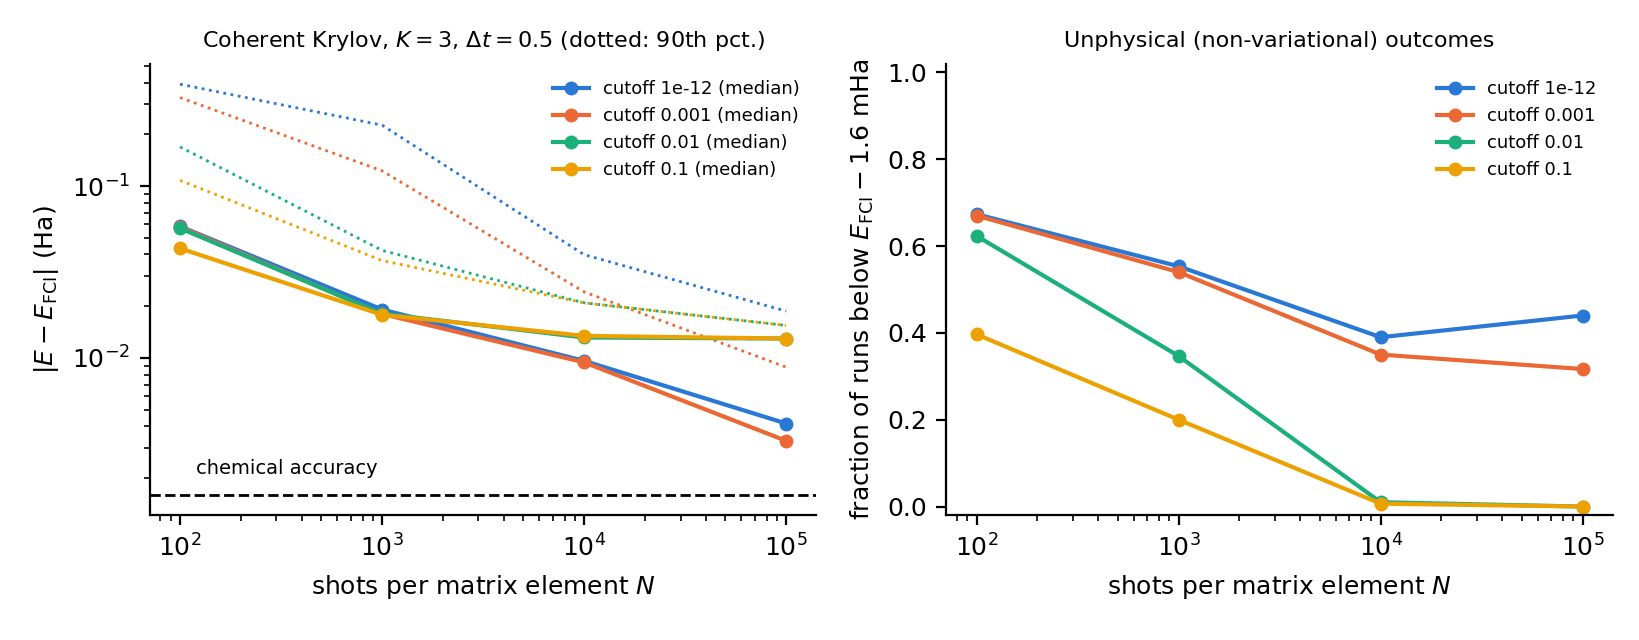
\includegraphics[width=\linewidth]{figures/krylov-conditioning-h2.png}
\caption{Check~B: toy coherent-Krylov on 2-qubit H$_2$ ($K=3$, $\Delta t=0.5$, 300 seeds per point). Left: median (solid) and 90th-percentile (dotted) absolute energy error versus shots per matrix element for four Gram cutoffs. Right: fraction of runs whose energy lies more than 1.6\,mHa \emph{below} the exact ground energy, i.e.\ unphysical outcomes caused by noise amplified through an ill-conditioned $\mathbf S$. Statevector toy with Gaussian shot noise; not a hardware result.}
\end{figure}
Reading: (i) with a weak cutoff, a third to a half of all runs land \emph{below} the true ground energy, which a variational method can never do; this is the ``negative-infinity energies'' failure \report\ describes (p.~4). (ii) A strong cutoff ($\ge10^{-2}$) removes the unphysical outcomes but collapses the rank to 1, i.e.\ to the HF energy (13\,mHa error): regularisation trades noise for bias. (iii) Even at $10^5$ shots per element, only a quarter of runs reach chemical accuracy at the best cutoff. On a 2-qubit model. This is the quantitative reason to prefer $\mathbf S=I$ sample-based methods or phase-estimation-type fits when the budget is small, and it is the first result a benchmark paper should show.

\subsection{Check C: sampled basis versus a classical-only control}
\lN\ Sampling bitstrings from the four Krylov states (10, 100 or 1024 shots each) always yields the support $\{\ket{01},\ket{10}\}$ and the exact energy. With 1\% simulated readout bit-flips the support grows to all four bitstrings; the energy is unchanged because the extra states lie in other symmetry sectors and cannot lower a variational energy. \textbf{The classical control, HF plus one connected shell under $H$ with no quantum sampling at all, gives the same support and the same exact energy.} This is flaw F7 in miniature: when the expansion saturates the sector, sampling is redundant. \report's active spaces are larger, but not large enough for the argument to change.

\subsection{Check D: arithmetic in the report}
\lN\ HQC (F19): Eq.~(9) as printed with $N_{2Q}=5436$, $N_{\rm meas}=12$, 1024 shots gives 11,266 ($N_{1Q}=0$) to 13,493 ($N_{1Q}=2N_{2Q}$) HQC per circuit, not 16,568; the printed 16,568 equals $5436\times1024/336$; the printed batch total $82{,}862.17$ divided by 6 is 13,810 and divided by 5 is 16,572. With the published formula $5+C(N_{1q}+10N_{2q}+5N_m)/5000$ \lV\ and $N_{1q}=N_{2q}$, the cost is 12,264 HQC per circuit. ``Survival fidelity'' (F17): $(1-p)^{5436}=3\times10^{-4}\Rightarrow p=1.49\times10^{-3}$, and $(1-p)^{150}=0.80$, $(1-p)^{204}=0.74$.

\subsection{Check E: statistical phase estimation versus coherent Krylov on the same data}\label{sec:checkE}
Both methods consume the signal $s(t_k)=\bra{\psi_0}e^{-iHt_k}\ket{\psi_0}$ on a time grid; coherent Krylov additionally needs $h(t_k)=\bra{\psi_0}He^{-iHt_k}\ket{\psi_0}$. \lN\ $K=24$ points at $\delta t=0.3$, Gaussian noise of standard deviation $1/\sqrt N$ on $\operatorname{Re}$ and $\operatorname{Im}$ of every point ($\lambda/\sqrt N$ for $h$, treating $H$ as one measurable, which is \emph{optimistic} for Krylov), 300 repetitions. SPE uses the matrix-pencil method with rank 2 (the toy signal has exactly two components, which favours SPE; see the caveat); Krylov uses $K/2=12$ basis states and a relative threshold of $10^{-3}$ on $\mathbf S$.

\begin{figure}[ht]\centering
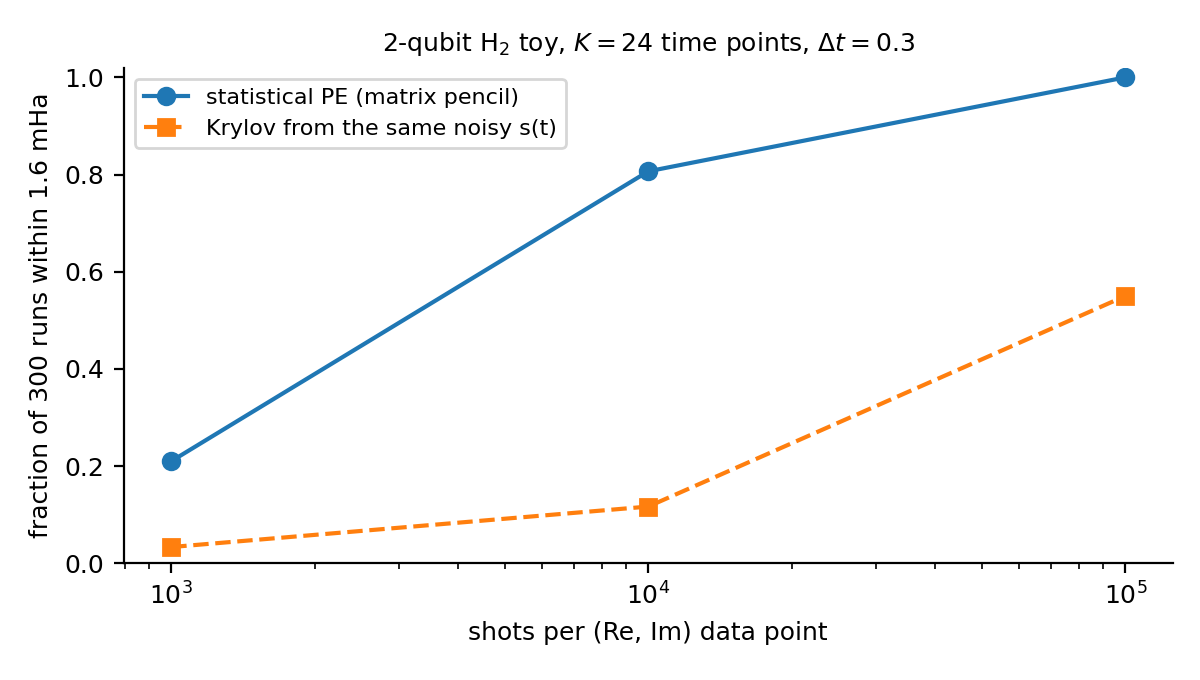
\includegraphics[width=.62\linewidth]{figures/spe-vs-krylov-h2.png}
\caption{Check~E: fraction of 300 noisy runs within chemical accuracy, two-qubit H$_2$ toy. Statistical PE (matrix pencil) and coherent Krylov are fed the same noisy survival signal; Krylov also gets the noisy $H$-weighted signal.}
\end{figure}

\begin{center}\footnotesize
\begin{tabular}{@{}lrrrrrr@{}}
\toprule
& \multicolumn{3}{c}{Statistical PE} & \multicolumn{3}{c}{Coherent Krylov, same data}\\
\cmidrule(lr){2-4}\cmidrule(lr){5-7}
Shots per point & median $|\Delta E|$ & within $1.6\mHa$ & below $E_0$ & median $|\Delta E|$ & within $1.6\mHa$ & below $E_0$\\\midrule
$10^3$ & $4.2\mHa$ & 21\% & 53\% & $46\mHa$ & 3\% & 78\%\\
$10^4$ & $0.85\mHa$ & 81\% & 8\% & $7.3\mHa$ & 12\% & 65\%\\
$10^5$ & $0.25\mHa$ & 100\% & 0\% & $1.4\mHa$ & 55\% & 26\%\\
\bottomrule
\end{tabular}
\end{center}

\textbf{Reading the table.} (i) For the same noisy data, fitting frequencies is far more shot-efficient than solving the generalised eigenproblem: at $10^4$ shots per point SPE is within chemical accuracy four times out of five, Krylov one time in eight. (ii) Krylov's failures are mostly \emph{non-variational} (energies below $E_0$), the signature of noise amplified by small eigenvalues of $\mathbf S$ (as in Check~B); SPE errors are symmetric and shrink with $N$. (iii) At $10^5$ shots per point and 24 points the total is $4.8\times10^6$ shots of Hadamard-test circuits; at 300 two-qubit gates that is roughly $3.5\times10^5\,\HQC$ (Check~G), i.e.\ seventy times a 5\,000 HQC budget. Both methods need \emph{much} shorter circuits or far fewer points on hardware; the sample-based arm exists precisely because it has no Hadamard tests.

\begin{caution}[Caveats of Check E]
Two components in the signal and a known rank make matrix pencil look better than it will on a real molecule, where the rank and the number of points must be chosen and QCELS-type least-squares fitting of the dominant frequency is the robust choice \lG. Krylov was given an optimistic noise model for $h(t)$ and a fixed threshold; a tuned threshold narrows the gap but does not close it (Check~B). None of this is a hardware statement.
\end{caution}

\subsection{Check F: how long an iterative-QPE circuit is}
\lN\ Kitaev's iterative phase estimation on the exact ground state of the toy (so that only the depth question is tested), energy window $[-2,0]\Ha$, 12 bits, 50 shots per bit: the estimate is $E_0$ to $0.15\mHa$, below chemical accuracy, as it should be. The price is that the round for the least-significant bit applies the unit evolution $2^{11}=2048$ times coherently, and the $m$-th bit $2^{m-1}$ times. On hardware each unit is a full Trotter step of the tapered Hamiltonian (hundreds of two-qubit gates); at $10^{-3}$ error per gate the survival probability of a $2048$-step circuit is zero for every practical purpose. This is the quantitative content of \cref{sec:p1}.

\subsection{Check G: HQC envelope for one 8-qubit instance}
\lN\ Arithmetic from the published formula $\HQC=5+C(N_{1q}+10N_{2q}+5N_m)/5000$ with $N_{1q}=2N_{2q}$ and $N_m$ = number of measured qubits:
\begin{center}\small
\begin{tabularx}{\linewidth}{@{}L{4.6cm}rrrY@{}}
\toprule
Circuit type & $N_{2q}$ & shots & HQC/circuit & Comment\\\midrule
Sampling circuit (sample-based arm) & 150 & $10^3$ & 373 & no ancilla; $\sim13$ circuits fit in 5\,000 HQC\\
Hadamard test (coherent Krylov, SPE) & 300 & $10^3$ & 734 & $\sim6$ time points per 5\,000 HQC\\
Hadamard test & 300 & $10^4$ & 7\,295 & one point exhausts the budget\\
QITE prefix after several steps & 600 & $10^3$ & 1\,453 & grows with step count\\
SPE, 24 points, Re and Im & 300 & $10^4$ each & 350\,160 total & Check~E at its best setting\\
\bottomrule
\end{tabularx}
\end{center}
The envelope says what the emulator stage must establish before hardware: how few time points and shots each arm can survive on. Checks~B and E suggest that the Hadamard-test arms need $\ge10^4$ shots per point for chemical accuracy, which is incompatible with a 5\,000 HQC budget at 300 two-qubit gates. Either the circuits must be an order of magnitude shorter (smaller instance, tapering, compiled gadgets) or the hardware budget must be an order of magnitude larger; this is the first go/no-go question of the strategy.

\takeaway{The toy confirms both halves of \report's central argument -- coherent Krylov is shot-hungry and non-variational under noise, and $\mathbf S=I$ removes that problem -- but also its central weakness: at small size the classical expansion alone gives the answer. It adds two facts the brief lacks: phase-estimation-type fitting of the same data is far more shot-efficient than the eigenproblem, and iterative QPE is a depth problem, not a qubit problem.}

%=====================================================================================
\clearpage
\part{Alternatives and strategy}

\section{Alternative and complementary approaches}\label{sec:alternatives}
For each approach: the idea, expected benefit relative to \report's compact-driver SKQD, cost, risk, and which Quantinuum features it exploits (hardware facts as in \cref{sec:hardware}).

\subsection*{A1. Sample-based diagonalisation done properly (SQD/QSCI with configuration recovery)}
\emph{Idea.} Keep the $\mathbf S=I$ structure but sample from a state with real correlation content (a truncated UCC or an ADAPT/Hiverge-grown circuit, or a full-$H$ Trotter state) and use the IBM-style configuration-recovery loop: estimate orbital occupations from the current Ritz vector, repair bitstrings that violate the sector, resample subspaces, iterate classically. \emph{Benefit.} Removes the arbitrary frequency filter (F6), gives an established name and citation base (F24), scales to 30--60 qubits where the expansion cannot saturate (F7). \emph{Cost.} Deeper state-preparation circuits ($10^2$--$10^3$ 2Q gates); classical eigensolves of $10^4$--$10^6$ dimension. \emph{Risk.} Already heavily published by IBM on superconducting hardware; novelty must come from the trapped-ion angle (fidelity allows deeper preparation; all-to-all removes SWAP overhead) and from the controls. \emph{Quantinuum features.} High 2Q fidelity, all-to-all connectivity, 56--98 qubits, InQuanto for Hamiltonians.

\subsection*{A2. Full-driver SKQD with the convergence guarantee, plus adaptive sampling}
\emph{Idea.} Evolve under the full tapered $H$ (first-order Trotter, few steps), so that Yu et al.'s theorem applies; allocate shots across time points with the marginal-discovery rule in your notes; select configurations by residual coupling to the current Ritz vector rather than by HF coupling. \emph{Benefit.} Turns the heuristic into a method with a statement; directly fixes F1, F5, F6. \emph{Cost.} More 2Q gates per circuit than the compact driver (all $\approx200$ pruned terms); 1 or 2 extra classical rounds for adaptive allocation. \emph{Risk.} Gives up part of the ``single batch'' argument if allocation is adaptive; may show that the driver choice does not matter at small size (a result in itself). \emph{Quantinuum features.} Nexus batching, all-to-all (Trotter of long Pauli strings without routing), emulators for the pilot.

\subsection*{A3. QITE and QITE-generated Lanczos (your existing arm)}
\emph{Idea.} Iteratively fit a unitary to each imaginary-time step from measured $S$ and $b$ (Motta et al.\ 2020); then use the QITE states at several $\tau$ as a Krylov (QLanczos) basis. \emph{Benefit.} A genuinely different algorithmic family (filter instead of subspace), gives a prepared state not just an energy, and the QLanczos variant yields a coherent Krylov arm whose basis is by construction well-conditioned in the direction of the ground state. Your \texttt{qite\_h2.py} already shows the shot-noise/ridge trade-off ($10^3$ shots: 151\,mHa plateau; $10^5$ shots: 2\,mHa; ridge $0.1$ rescues $10^3$ shots to 17\,mHa). \emph{Cost.} Many sequential rounds (each needs the device), circuit depth grows with steps, and the pool size grows exponentially with domain size. \emph{Risk.} Cloud latency per round; on $>8$ qubits the local-domain approximation may stall. \emph{Quantinuum features.} High fidelity for accumulated depth; conditional logic/real-time feedback could in principle run small QITE updates inside one job (to verify whether Nexus supports classical linear solves in-loop; Helios advertises a real-time control engine).

\subsection*{A4. Coherent quantum Krylov with error-detected Hadamard tests}
\emph{Idea.} Measure $\mathbf S$ and $\mathbf H_K$ with a single ancilla, exploiting the Toeplitz structure (only $K$ distinct elements, not $K^2$), and protect the ancilla and register with mid-circuit symmetry checks (particle number, parity) that discard faulty shots; reset and reuse the ancilla between elements. \emph{Benefit.} The ``prohibitive'' controlled-Trotter cost (F12) is far smaller after tapering/pruning (a 200-term step on 8 qubits is a few hundred 2Q gates, feasible at 99.9\%); and it provides the honest coherent-Krylov baseline \report\ lacks. \emph{Cost.} Shots: Checks~B and E say $10^4$--$10^5$ per element for chemical accuracy; post-selection multiplies cost by $1/(\text{acceptance})$. \emph{Risk.} Conditioning: needs a declared regularisation policy; may simply lose to A1/A2 at fixed budget (which would be a clean result). \emph{Quantinuum features.} Mid-circuit measurement, qubit reuse, conditional operations, all-to-all (controlled Pauli gadgets without routing).

\subsection*{A5. Short-circuit phase estimation (RPE / QCELS-type)}
\emph{Idea.} Estimate $E_0$ from the time series $\braket{\psi_0}{e^{-iHt}\psi_0}$ measured with one ancilla, using robust phase estimation or least-squares fitting of a few complex exponentials (QCELS); no eigenproblem, no $\mathbf S$. \emph{Benefit.} Heisenberg-limited shot scaling and provable error bounds given overlap $|\braket{\psi_0}{E_0}|^2>1/2$; the natural ``QPE-lite'' arm; on the toy it is $4$--$7\times$ more likely to reach chemical accuracy than Krylov from the same data (Check~E). \emph{Cost.} Controlled evolution for several $t$, deeper than Krylov at the longest $t$; but the data are the same Hadamard-test circuits as A4, so as a fourth arm it is free. \emph{Risk.} Overlap requirement fails for strongly correlated instances; depth. \emph{Quantinuum features.} High fidelity, ancilla reuse; same error-detection as A4. (Verify the specific QCELS/RPE references before citing.)

\subsection*{A6. Observable dynamic mode decomposition / filter diagonalisation}
\emph{Idea.} Use the same time series as A5 but extract eigenvalues by DMD or filter diagonalisation (Hankel-matrix methods, as the matrix pencil in Check~E), which are known to be robust to noise and to ill-conditioning through rank truncation. \emph{Benefit.} Reuses A5 data; gives excited states too. \emph{Cost.} None beyond A5. \emph{Risk.} Newer literature (Shen et al.\ 2023, to verify); fewer hardware demonstrations. \emph{Quantinuum features.} as A5.

\subsection*{A7. ADAPT-VQE / Hiverge-discovered ansatz as the Quantinuum-native baseline}
\emph{Idea.} Use the Hiverge paper's own evolved \texttt{generate\_ansatz()} routines (public repository) or standard ADAPT-VQE as (i) the variational baseline and (ii) the state-preparation circuit for sampling in A1. \emph{Benefit.} Immediate credibility and a natural collaboration hook with the Hiverge/InQuanto team; the H$_2$O 14-qubit and F$_2$ 20-qubit instances already have published resource counts to compare against. \emph{Cost.} Classical optimisation ($10^3$--$10^4$ evaluations) before hardware. \emph{Risk.} Not novel on its own (\cref{sec:p3}). \emph{Quantinuum features.} InQuanto pools, CUDA-Q emulation, H2 native compilation.

\subsection*{A8. Error detection with mid-circuit measurement}
\emph{Idea.} Beyond PMSV post-selection, encode the register in a lightweight detection code (the Iceberg $[[k+2,k,2]]$ code demonstrated on H-series by Self et al.\ 2024, to verify) or use ancilla-mediated particle-number checks at intervals, discarding shots that flag an error. \emph{Benefit.} Converts hardware noise into a known acceptance rate instead of unknown bias; a distinctive trapped-ion capability that superconducting SQD papers cannot match (\cref{sec:p4}). \emph{Cost.} 2 extra qubits and some 2Q gates per check; shots divided by acceptance. \emph{Risk.} Overhead may exceed benefit at 8--16 qubits; needs Quantinuum compiler support. \emph{Quantinuum features.} Mid-circuit measurement, conditional logic, qubit reuse, all-to-all.

\subsection*{A9. Qubit-efficient and symmetry-adapted encodings}
\emph{Idea.} Tapering (already used); seniority-zero / paired encodings (one qubit per spatial orbital) for near-equilibrium cases; qubit-efficient CI encodings that map $D$ determinants to $\lceil\log_2D\rceil$ qubits (Yoffe et al.\ 2025, cited by Hiverge as ref.~72). \emph{Benefit.} Larger active spaces at the same qubit count; sector violations become impossible by construction. \emph{Cost.} Non-local Hamiltonians; more complex circuits. \emph{Risk.} Paired encodings lose accuracy at dissociation. \emph{Quantinuum features.} All-to-all connectivity makes non-local encodings cheap.

\subsection{Comparison and ranking}
Scores are my judgement \lA\ on a 1--5 scale (5 = best). ``Novelty'' is novelty of a paper built around the item with Quantinuum; ``Feasibility'' is within $\sim$4 months with emulator access and a modest hardware budget.
\begin{center}\small
\begin{tabularx}{\linewidth}{@{}lYcccY@{}}
\toprule
ID & Approach & Novelty & Feasib. & Shot cost & Hardware feature exploited\\\midrule
A1 & SQD/QSCI with recovery, deep prep & 3 & 4 & low & fidelity, all-to-all, qubit count\\
A2 & Full-driver SKQD + adaptive shots + residual selection & 4 & 5 & low & batching, emulators\\
A3 & QITE / QLanczos & 3 & 3 & high & fidelity for depth; real-time control (verify)\\
A4 & Error-detected coherent Krylov & 4 & 3 & high & mid-circuit meas., reuse, conditional ops\\
A5 & RPE / QCELS (free fourth arm on A4 data) & 3 & 4 & medium & fidelity, ancilla reuse\\
A6 & ODMD / filter diagonalisation & 4 & 3 & medium & as A5\\
A7 & ADAPT / Hiverge ansatz baseline & 1 & 5 & medium & InQuanto, emulators\\
A8 & Iceberg / symmetry error detection & 4 & 3 & medium & mid-circuit meas., conditional logic\\
A9 & Qubit-efficient encodings & 3 & 4 & low & all-to-all\\
\bottomrule
\end{tabularx}
\end{center}
\textbf{Ranking for the paper.} The combination with the best novelty-times-feasibility is a \textbf{four-arm, budget-matched benchmark}: A2 (sample-based arm, with classical controls) versus A4 (coherent Krylov arm with error detection) versus A3 (QITE/QLanczos arm, your existing work) versus A5 (statistical phase estimation, computed from the A4 data at no extra hardware cost), with A7 as state preparation and baseline, and A8 as the hardware-specific ingredient that distinguishes the paper from IBM's SQD line. A6 is an optional post-processing variant of A5.

\subsection{Verdict table for the brief's paradigms}
\begin{center}\small
\begin{tabularx}{\linewidth}{@{}L{3.1cm}YL{2.3cm}L{2.9cm}@{}}
\toprule
Paradigm (brief) & Role in our paper & Hardware feature used & Status of the brief's description\\\midrule
1. QPE + DF/THC, IQPE & One row in a cost table (``what full QPE would need''); no runs & none (fault-tolerant) & correct as road map, irrelevant to the budget; ``no loss of precision'' hides $2^m$ depth\\
2. Krylov / QLanczos & Backbone: sample-based arm (A2) and coherent arm (A4); QLanczos on top of QITE (A3) & all-to-all; MCMR for ancilla reuse and checks & correct method; ``Quantinuum favours it'' unsupported; swap-network sentence backwards; cost and conditioning omitted\\
3. ADAPT / generative & State preparation and variational baseline (A7), optimised on the emulator & emulators, InQuanto, native compilation & ADAPT correct; ``transformer, 10$\times$'' conflates Hiverge with GQE, unsourced\\
4. Logical GSEE / SPE / syndromes & SPE as fourth arm (A5, free from the A4 data); error detection (A8) as the hardware-specific ingredient; logical qubits out of scope & MCMR, conditional logic, qubit reuse & SPE correct and near-term; logical-qubit claims partly unverifiable; syndromes $\ne$ symmetry checks\\
\bottomrule
\end{tabularx}
\end{center}

\takeaway{No single algorithm is the ``better'' one; the publishable object is the comparison under identical budgets, with the hardware's mid-circuit measurement used for error detection in the arms that need an ancilla.}

\section{Future strategy: a publishable paper with Quantinuum}\label{sec:strategy}

\subsection{Central research question and claims}
\begin{idea}[Research question]
For a fixed molecular Hamiltonian, sector and reference, and a fixed hardware budget (shots, shot-weighted two-qubit gates, HQCs, wall time), which of four ground-state strategies -- sample-based diagonalisation (SKQD/SQD), coherent real-time Krylov with error-detected overlaps, imaginary-time filtering (QITE/QLanczos), and statistical phase estimation on the same overlap data -- reaches a target accuracy most reliably, and in which regime (system size, correlation strength) does the quantum sampling contribute beyond classical selection?
\end{idea}
Publishable claims this can support (pre-registered as hypotheses, not outcomes):
\begin{enumerate}
\item A \textbf{regime map}: at $\le8$ tapered qubits the classical expansion alone reaches chemical accuracy (confirming F7); at 16--24 qubits with strong correlation, quantum-seeded selection reaches a given error with a $D$ that is $X\times$ smaller than HF-seeded or random-seeded selection at the same classical cost.
\item A \textbf{cost frontier}: error versus cumulative HQC (and versus shot-weighted 2Q gates) for the four arms, with confidence intervals, on the same instances.
\item A \textbf{hardware-specific result}: mid-circuit symmetry/error detection improves the coherent-Krylov and SPE arms' variational reliability (fraction of non-variational outcomes) at a quantified acceptance cost.
\item A \textbf{same-data result}: on identical Hadamard-test shots, phase-estimation-type fitting versus the generalised eigenproblem (Check~E made quantitative on 8--16 qubits).
\item A \textbf{negative result is acceptable}: if sample-based always wins at these sizes, the paper reports that with the numbers; the Hiverge paper's LiH hardware point is an example of a modest hardware result published honestly.
\end{enumerate}

\subsection{Work packages}
\textbf{WP0 -- Reproduce and control (weeks 1--3, simulator only).} Rebuild \report's H$_2$O CAS(8e,6o) and F$_2$ CAS(10e,6o) pipelines in statevector (PySCF/InQuanto for integrals, your own tapering code validated against the sector spectrum). Run: quantum-seeded expansion vs.\ HF + $s$ shells vs.\ random valid-sector seeds, all at matched final $D$. \emph{Metrics:} error vs.\ $D$; external residual. \emph{Go/no-go:} if no quantum-seeded case beats the HF-seeded control at matched $D$ (expected), record it and move to larger instances; if one does, keep that instance.

\textbf{WP1 -- Freeze the problem set and budgets (weeks 2--5).} Choose three instances with a classical reference and increasing difficulty, e.g.\ H$_2$O CAS(8e,6o) (continuity with \report, 8 qubits), N$_2$ at $R\in\{1.1,1.6,2.2\}$\,\AA\ in CAS(10e,10o) or CAS(10e,12o) (20--24 qubits before tapering; strongly multireference at stretch), and one 14--16-orbital case with a DMRG/SHCI reference (e.g.\ a larger-basis H$_2$O or a benzene $\pi+\sigma$ space; to be chosen with Quantinuum's chemists). Freeze geometry, basis, active orbitals, sector, energy offset, HF reference. Define three budgets $B\in\{10^4,10^5,10^6\}$ total shots and the corresponding HQC and 2Q-gate-shot totals (Check~G is the template); publish the allocation policy for each arm before any run. Deliverable: a machine-readable manifest with Hamiltonian hashes (your notes' template).

\textbf{WP2 -- Four arms in simulation (weeks 4--10).} Stage A exact statevector; Stage B shot noise only (independent whole-algorithm repeats, $\ge50$ seeds); Stage C H2-1E/H2-2E noise model with raw / sector post-selection / PMSV; Stage C$'$ forecast model with improved error rates (as Hiverge Fig.~7). Arms: (i) SKQD/SQD with full-$H$ Trotter driver, adaptive shots, residual selection, plus \report's compact driver as an ablation; (ii) coherent Krylov, $K\le6$, Toeplitz measurement, declared cutoff policy, with and without mid-circuit symmetry checks; (iii) QITE with $\Delta\tau\in\{0.02,0.05,0.1\}$, two pools, ridge/cutoff policy, and QLanczos on its states; (iv) statistical PE (QCELS-type fit, not a fixed-rank pencil) on the arm-(ii) time series, with the number of time points and shots per point as the tuning knobs. ADAPT/Hiverge ansatz as baseline and as starting state. \emph{Metrics:} median and IQR of error, $P(\text{chem.\ acc.})$, non-variational fraction, $D$, residual, per-circuit 2Q/depth, total shots, HQC estimate, classical time. \emph{Go/no-go for hardware:} an arm goes to hardware on an instance only if $P(\text{chem.\ acc.})\ge0.8$ on the emulator at the chosen budget, or if its failure is itself the finding (then one confirmatory run). The first go/no-go question is the one Check~G poses: can the Hadamard-test arms reach chemical accuracy with few enough points and shots to fit the budget at all?

\textbf{WP3 -- Hardware (weeks 8--14).} Design: for each (instance, arm, budget) that passed WP2, three independent jobs interleaved across arms within the same calibration window; $10^4$ shots per circuit where affordable (Hiverge standard); error-detected variants of arms (ii) and (iv) and sector post-selection for all; raw and mitigated results stored separately. Record device, date, calibration snapshot, pytket/InQuanto/Nexus versions, HQCs charged, QPU and queue time, every raw count file. Expected hardware scale: $8$--$16$ tapered qubits, $\le300$ 2Q gates per circuit, $10$--$40$ circuits per arm-instance; total HQC to be estimated with the official calculator before submission.

\textbf{WP4 -- Analysis and paper (weeks 12--18).} Bootstrap all hardware results; produce the figures below; ablation ladder for the sample-based arm (driver / filter / selection / shells); reconcile emulator forecasts with hardware; write with Quantinuum co-authors; release code and data.

\subsection{Figures the paper needs}
\begin{enumerate}
\item \textbf{Central figure: error versus cumulative hardware cost.} $x$ = cumulative HQC (second panel: shot-weighted 2Q gates), $y$ = $|E-E_{\rm ref}|$ on a log scale with bootstrap intervals; one line per arm; chemical-accuracy line; classical controls as horizontal references; hardware points as stars over emulator curves (Hiverge Fig.~7 style). One panel per instance.
\item Probability of chemical accuracy versus budget, per arm.
\item Quantum-seeded versus classical-seeded selection: error versus final dimension $D$ (the F7 test); this figure decides whether the sampling matters.
\item Mechanism/ablation ladder for the sample-based arm (driver, filter, selection, shells), Hiverge Fig.~6 style.
\item Non-variational fraction and retained rank versus shots and cutoff for coherent Krylov, with and without error detection; SPE from the same data on the same axes (hardware-specific and same-data results).
\item Resource ledger table: per circuit and per arm, 2Q gates, depth, shots, HQC, QPU time, classical time, memory.
\end{enumerate}

\subsection{Statistics}
Report medians and interquartile ranges over independent repeats, bootstrap confidence intervals over shots within a job, $P(\text{chem.\ acc.})$ with a Wilson interval, and signed errors (to show non-variational outcomes). Pre-register thresholds, cutoffs and allocation policies in the WP1 manifest. Use held-out geometries for any threshold tuned on data. Never compare a statevector curve to a hardware cost axis.

\subsection{Timeline, risks and mitigations}
\begin{center}\small
\begin{tabularx}{\linewidth}{@{}lYY@{}}
\toprule
Weeks & Milestone & Risk and mitigation\\\midrule
1--3 & WP0 controls done; decision on instance set & Classical control wins everywhere at 8 qubits: expected; this is Fig.~3, not a failure\\
2--5 & WP1 manifest frozen; budgets and HQC estimates agreed with Quantinuum & Reference for the 14--16-orbital case unavailable: use DMRG/SHCI via a collaborator, or shrink to 12 orbitals\\
4--10 & WP2 emulator results for all arms & QITE stalls or is too deep at 16+ qubits: report it, keep QLanczos on fewer steps; Hadamard-test arms too shot-hungry (Check~G): keep one instance only, or shorten circuits\\
8--14 & WP3 hardware campaign & Budget overrun: fix $B$ per arm in advance, prioritise the central figure's points; drift: interleave arms, repeat the HF-only circuit as a control each session\\
12--18 & WP4 paper and data release & Results modest: frame as cost frontier and regime map; emphasise the error-detection and same-data results\\
\bottomrule
\end{tabularx}
\end{center}

\subsection{Collaboration and authorship with Quantinuum}
Approach the InQuanto/applications group that co-authored the Hiverge paper (the preprint names InQuanto, emulator and hardware-execution staff in its acknowledgements). Offer: a benchmark design, the classical controls and the QITE arm; ask for: emulator access with the current noise model and PMSV, help with compilation and mid-circuit-measurement constructs, hardware time, and a chemist's choice of the 14--16-orbital instance. Agree authorship early (contribution statement per WP), data-release terms and whether the hardware specification source can be cited. \report's author should be invited as co-author for the SKQD arm; the existing water/F$_2$ job data become WP0 inputs if released.

\subsection{Candidate venues (suggestions)}
arXiv (quant-ph) first. Then, depending on the outcome: \emph{PRX Quantum} or \emph{Quantum} for a methods-plus-hardware benchmark; \emph{npj Quantum Information} or \emph{Physical Review Research} for a solid but modest hardware result; \emph{J.~Chem.\ Theory Comput.}\ or \emph{J.~Chem.\ Phys.}\ if the chemistry (regime map, classical controls) is the main story. A Quantinuum technical note or blog can accompany the preprint.

\subsection{What \emph{not} to put in the paper}
QPE runs; DF/THC implementations; logical-qubit experiments; a generative-ansatz claim we did not produce; any ``supremacy'' language; any cost quoted in dollars rather than compiled gate counts and HQC; any statevector curve on a hardware cost axis.

\takeaway{The paper is the comparison, not any one method. Freeze the problem, pre-register budgets, run controls first, go to hardware only with emulator evidence, and report cost and uncertainty like the Hiverge paper.}

\clearpage
\section{Action checklist}\label{sec:checklist}
\textbf{Before any new computation}
\begin{itemize}
\item[$\square$] Ask \report's author for the WP0 inputs: tapered Hamiltonians, driver lists, compiled circuits, raw per-circuit counts, filter/expansion code, exact reference energies (your notes' request list).
\item[$\square$] Rewrite the brief's four sections with the corrections in \cref{sec:p1,sec:p2,sec:p3,sec:p4,sec:pipeline} before it is used in any proposal (the Hiverge/GQE conflation, the swap-network sentence, the $10^{-4}$ error figure, the logical-qubit code list, the ``halving'' claim).
\item[$\square$] Cite Yu et al.\ 2025 (SKQD), Robledo-Moreno et al.\ 2025 (SQD), Kanno et al.\ 2023 (QSCI), Motta et al.\ 2020 (QITE/QLanczos), Stair et al.\ 2020 (multireference QKS), Ding and Lin 2023 (QCELS); verify each reference.
\item[$\square$] Replace Eq.~(9) by the published HQC formula; recompute all costs; never quote HQCs as dollars.
\end{itemize}
\textbf{Classical controls (WP0)}
\begin{itemize}
\item[$\square$] HF + $s$ shells and random-seed expansions at matched $D$ for H$_2$O and F$_2$; plot error vs.\ $D$.
\item[$\square$] Record $|\braket{\mathrm{HF}}{E_0}|^2$, gap, weight distribution and sector dimension for every instance.
\item[$\square$] Reproduce the 0.1836\,mHa statevector residual for water and explain it.
\end{itemize}
\textbf{Design freeze (WP1)}
\begin{itemize}
\item[$\square$] Three instances, references, sectors, offsets, HF reference, Hamiltonian hashes in a manifest.
\item[$\square$] Budgets $B$ and allocation policy per arm, pre-registered; thresholds and cutoffs fixed or tuned only on held-out geometries.
\item[$\square$] HQC ledger for every circuit type on the chosen instances (Check~G as template); decide the budget tiers.
\end{itemize}
\textbf{Simulation (WP2)}
\begin{itemize}
\item[$\square$] Extend \texttt{code/qite\_h2.py} and \texttt{code/krylov\_toy\_checks\_h2.py} to 8 qubits (H$_4$ or LiH) with a Trotterised propagator and compiled gate counts; rerun Check~E with QCELS-type fitting.
\item[$\square$] Stage A/B/C/C$'$ for all four arms; $\ge50$ whole-algorithm seeds; raw / sector post-selection / PMSV.
\item[$\square$] Ablations: driver size, filter variants, selection rule, shells; QITE $\Delta\tau$ and pool; Krylov $K$, $\Delta t$, cutoff, with/without error detection; SPE points and shots per point.
\item[$\square$] Design the mid-circuit checks (parity or Iceberg) once and apply identically to arms (ii), (iii), (iv).
\item[$\square$] Go/no-go per (instance, arm): $P(\text{chem.\ acc.})\ge0.8$ on emulator or a declared confirmatory run.
\end{itemize}
\textbf{Hardware (WP3)}
\begin{itemize}
\item[$\square$] Three interleaved jobs per point; $10^4$ shots per circuit where affordable; HF-only control circuit each session.
\item[$\square$] Log device, date, calibration, software versions, HQC charged, QPU and queue time, all raw counts.
\item[$\square$] Store raw and mitigated results separately; bootstrap intervals for everything.
\end{itemize}
\textbf{Paper (WP4)}
\begin{itemize}
\item[$\square$] Figures 1--6 of \cref{sec:strategy}; provenance column in every table; resource ledger.
\item[$\square$] Limitations paragraph; one-sentence scope statement excluding QPE and logical qubits; no ``supremacy'', ``scalable'' or ``100\% pass rate'' without a defined population.
\item[$\square$] Public repository with code, manifests, counts and an environment file; authorship and data terms agreed with Quantinuum.
\item[$\square$] Verify every \lG\ item in this document before it is cited.
\end{itemize}

\section*{References}
\addcontentsline{toc}{section}{References}
{\sloppy\textbf{Sources read for this document (verified):} the report under review (A.~Kumar, ``Scalable Non-Iterative Quantum Krylov Subspace Chemistry on Trapped-Ion Processors'', 8 Oct 2026, 14 pp.); Finger, Rapp, Kalidindi et al.\ (Quantinuum/Hiverge), ``Automated near-term quantum algorithm discovery for molecular ground states'', arXiv:2603.26359 (27 Mar 2026); Quantinuum System Model H2 product page and Nexus job-costing documentation (accessed 15 Oct 2026, HQC formula $5+C(N_{1q}+10N_{2q}+5N_m)/5000$); the project documents \texttt{Krylov\_SKQD\_Study\_Notes.tex}, \texttt{qite-complete-guide.tex}, \texttt{code/qite\_h2.py} and \texttt{code/results.json}.\par}

\textbf{Literature cited from memory, \alert{to verify before use in a manuscript}:}
\begin{itemize}\small\sloppy
\item Yu, Robledo-Moreno et al., ``Quantum-centric algorithm for sample-based Krylov diagonalization'', arXiv:2501.09702 (2025) (SKQD).
\item Robledo-Moreno et al., ``Chemistry beyond the scale of exact diagonalization on a quantum-centric supercomputer'', Science Advances (2025), arXiv:2405.05068 (SQD).
\item Kanno et al., ``Quantum-selected configuration interaction'', arXiv:2302.11320 (2023) (QSCI).
\item M.~Motta et al., Nature Physics 16, 205 (2020) (QITE/QLanczos; report ref.~[4]); W.~Kirby et al., ``Exact and efficient Lanczos method on a quantum computer'', Quantum 7, 1018 (2023).
\item Stair, Huang, Evangelista, JCTC 16, 2236 (2020) (multireference QKS; report ref.~[3]); Bravyi, Gambetta, Mezzacapo, Temme, arXiv:1701.08213 (tapering; report ref.~[8]).
\item L.~Lin and Y.~Tong, ``Heisenberg-limited ground-state energy estimation for early fault-tolerant quantum computers'', PRX Quantum 3, 010318 (2022); Z.~Ding and L.~Lin, QCELS, PRX Quantum 4, 020331 (2023); Russo et al., robust phase estimation for energy differences (2021); Shen et al., observable dynamic mode decomposition (2023).
\item V.~von Burg et al., ``Quantum computing enhanced computational catalysis'', Phys.\ Rev.\ Research 3, 033055 (2021) (DF); J.~Lee et al., ``Even more efficient quantum computations of chemistry through tensor hypercontraction'', PRX Quantum 2, 030305 (2021) (THC).
\item H.~R.~Grimsley et al., ``An adaptive variational algorithm for exact molecular simulations on a quantum computer'', Nat.\ Commun.\ 10, 3007 (2019); H.~L.~Tang et al., ``qubit-ADAPT-VQE'', PRX Quantum 2, 020310 (2021); K.~Nakaji et al., ``The generative quantum eigensolver (GQE) and its application for ground state search'', arXiv:2401.09253 (2024).
\item C.~N.~Self, M.~Benedetti, D.~Amaro, ``Protecting expressive circuits with a quantum error detection code'', Nat.\ Phys.\ 20, 219 (2024) (Iceberg code on H-series); Yamamoto et al., PMSV, Phys.\ Rev.\ Research 4, 033110 (2022) (Hiverge ref.~70); Yoffe et al., qubit-efficient VSCI, QST 10, 015020 (2025) (Hiverge ref.~72).
\item A.~Cowtan et al., ``Phase gadget synthesis for shallow circuits'', EPTCS 318 (2020) (TKET gadget synthesis).
\end{itemize}

\end{document}
